\documentclass[12pt,fсeqn]{article}

%\usepackage[cp1251]{inputenc}
\usepackage[T2A]{fontenc}
%\usepackage{amssymb,amsmath,mathrsfs,amsthm}

\usepackage[footnotesize]{caption2}
\usepackage{indentfirst}
\usepackage{multicol}
%\usepackage[cp1251]{inputenc}
% %\usepackage[russian]{babel}
\usepackage{amssymb,amsmath}

%\usepackage[T2A]{fontenc}
\usepackage[utf8]{inputenc}
\usepackage{graphicx, graphics, epsfig}
\usepackage{epstopdf}
\usepackage{ifpdf}  
%\usepackage[scaled=.92]{helvet}
%\usepackage{times}
\usepackage{mathrsfs}
\usepackage{amsfonts}
\usepackage[english,russian]{babel}

\usepackage[pdftex,unicode]{hyperref}
%\usepackage[noend]{algorithmic}
\usepackage[noend]{algorithm}
\usepackage[noend]{algpseudocode}
\usepackage{hyperref}


\textheight=24cm
\textwidth=16cm
\oddsidemargin=5mm
\evensidemargin=-5mm
\marginparwidth=36pt
\topmargin=-1cm
\footnotesep=3ex
%\flushbottom
\raggedbottom
\tolerance 2000
% подавить эффект "висячих стpок"
\clubpenalty=10000
\widowpenalty=10000
%\renewcommand{\baselinestretch}{1.1}
\renewcommand{\baselinestretch}{1.5} %для печати с большим интервалом



\topmargin=-1.5cm


%\parindent=24pt
%\parskip=0pt
%\tolerance=2000
\flushbottom
%\def\baselinestretch{1.2} 

\author{Вишневский~Валерий~Викторович}

\begin{document}

\begin{titlepage}
\begin{center}
    Московский государственный университет имени М. В. Ломоносова

    \bigskip
    \includegraphics[width=50mm]{msu.eps}

    \bigskip
    Факультет Вычислительной Математики и Кибернетики\\
    Кафедра Математических Методов Прогнозирования\\[10mm]

    \textsf{\large\bfseries
        ДИПЛОМНАЯ РАБОТА СТУДЕНТА 517 ГРУППЫ\\[10mm]
        <<Параллельная реализация метода поиска закономерностей в последовательностях событий>>
    }\\[10mm]

    \begin{flushright}
        \parbox{0.5\textwidth}{
            Выполнил:\\
            студент 5 курса 517 группы\\
            \emph{Вишневский Валерий Викторович}\\[5mm]
            Научный руководитель:\\
            к.ф-м.н., н.с.\\
            \emph{Ветров Дмитрий Петрович}
        }
    \end{flushright}

%     \begin{tabular}{p{0.45\textwidth}p{0.45\textwidth}}
%         Заведующий кафедрой\newline
%         Математических Методов\newline
%         Прогнозирования, академик РАН
%         &
%         ~\newline~\newline
%         \hfill\hbox to 0.45\textwidth{\hrulefill~Ю. И. Журавлёв}
%     \\[20mm]
%         К защите допускаю\newline
%         \hbox to 0.4\textwidth{<<\hbox to 12mm{\hrulefill}>> \hrulefill~2010 г.}
%         &
%         К защите рекомендую\newline
%         \hbox to 0.45\textwidth{<<\hbox to 12mm{\hrulefill}>> \hrulefill~2010 г.}
%     \end{tabular}

    \vspace{\fill}
    Москва, 2011
\end{center}
\end{titlepage}


\newcommand{\evt}{ {\bf e} }
\newcommand{\pat}{ {\bf P} }
\newcommand{\Var}{\mathsf{var}}
\newcommand{\Erf}{\mathsf{erf}}

\begin{abstract}
В данной работе предлагается оригинальный алгоритм для поиска скрытых закономерностей(паттернов) в последовательностях событий,
основанный на вероятностном представлении паттернов в дискретных последовательностях событий. Также рассматривается 
применение данного алгоритма для анализа поведения мышей. Найденные паттерны используются для классификации
животных.

%В результате чего, по полученному множеству паттернов можно определить
%группу мышей, к которой относится наблюдаемая особь.

Проведено сравнение реализованного алгоритма с существующими аналогами, показавшее, что предложенный метод более устойчив к шуму в 
исходных данных и позволяет найти более значимые закономерности.
Приведен анализ параметров алгоритма. Предложенный метод поиска паттернов основывается на определении взаимосвязи между парами событий. 
Поиск производится снизу вверх: алгоритм сначала находит простые
закономерности, потом, путем соединения простых, образуются более сложные паттерны. 
На каждом шаге проводится отбор самых существенных и полных паттернов.

Данный алгоритм был реализован в среде \verb!Matlab!. Наиболее вычислительно-сложные процедуры были реализованы в виде 
\verb!mex!-файлов на языке \verb!C++!, с использованием технологии \verb!CUDA!. Параллельная реализация отдельных процедур
на \verb!GPU! дала ускорение в 20 и 140 раз по сравнению с последовательной версией на языке \verb!C++!.
\end{abstract}
\newpage
\tableofcontents
\newpage

\section{Введение}
Задача поиска закономерностей(стереотипов, паттернов, шаблонов~--- здесь синонимы) в поведении животных и людей крайне важна
в современной нейробиологии и когнитивных науках. Выделив характерные паттерны, мы, например, можем делать выводы
о сложности поведения различных особей, определять изменения в поведении наблюдаемых процессов,
другими словами, решив задачу поиска паттернов, мы можем определенным образом {\em измерять} поведение особи, или
группы особей, становится возможно более наглядно анализировать поведение.
Именно анализ поведения является основным инструментом при исследовании на системном уровне механизмов работы памяти и обучения животных.

В современной нейробиологии можно выделить три основных подхода к описанию поведения~\cite[с.~57]{Martin_Bateson}.
\begin{description}
 \item[Структурное описание:] определяет какие двигательные действия животное совершает в каждый момент времени. ( Неформально, можно сказать, что
для животного-робота, такое описание будет служить последовательностью инструкций, выполняя которые можно воспроизвести
какое-либо поведение).
\item[Эффектное описание:] определяет, какие эффекты имеет текущее поведение на само животное, или окружающую его среду, причем
сами физические действия субъекта, приведшие к определенному событию обычно не рассматриваются. При таком
подходе, поведения может описываться, например, следующими {\em терминами}: <<кормление>>, <<проявление агрессии>>,
<<сбор нектара>>, <<уход от хищника>>.
\item[Пространственное описание:] в данном случае, поведение животного описывается траекторией его движения во времени.
Это описание может быть усложнено, например, добавлением информации об ориентации животного, или о том, в каком темпе
производится движение(украдка, бег, и т.\,д.). В то же время, пространственное описание может быть упрощено, например,
клетка разбивается на несколько зон, после чего, подсчитывается время проведенное животным в каждой из зон.
\end{description}
 
Например, <<включить свет>>~--- это {\em поведенческий акт} в терминах эффектного описания, будет описано, как <<нажать на выключатель указательным пальцем>>
в терминах структурного описания.
 
Все три метода, по сути, описывают поведение, как некоторый процесс во времени. Можно заметить, что в первом и втором
случае поведение описывается <<более дискретно>>, поэтому обычно методы, применяемые для исследования пространственного описания
поведения, неприменимы для исследования структурного и эффектного описания, а для исследования структурного и эффектного описания
обычно используются одинаковые подходы.
 
Мы будем рассматривать случай, когда поведение описано в структурных или эффектных терминах. Тогда, в каждый момент
времени может происходить смена состояния, подразумевается, что начало текущего поведенческого акта совпадает
с концом предыдущего. Так мы можем записывать только моменты времени, когда поведенческий акт {\em начинается}.
Множество документируемых поведенческих актов определяется экспертами на этапе планирования эксперимента,
а сама разметка поведения на эти акты может производится по данным видеонаблюдения вручную, или
автоматически с помощью специализированного ПО, например, \verb!Noldus Observer!~\footnote{ \url{http://www.noldus.com/content/the-observer-xt}}.

\begin{figure}[H]
\noindent\centering{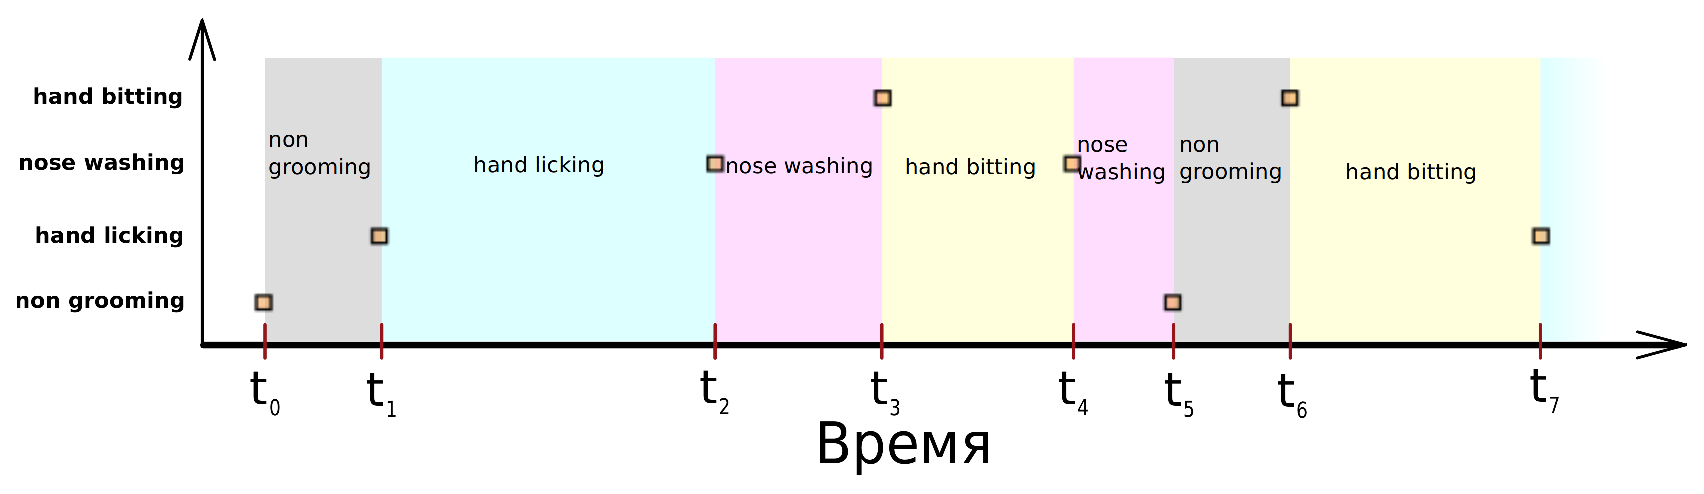
\includegraphics[width=163mm]{beh_data.eps}}
\caption{Пример описания поведения. По вертикали отложены фиксируемые поведенческие акты, по горизонтали~--- время. 
Начало каждого следующего акта является концом предыдущего. }
\end{figure}

Многие паттерны поведения являются тривиальными и понятными. В человеческом поведении, большинство повседневных церемоний,
ритуалов приветствия, рабочих и игровых процессов, по сути, являются поведенческими паттернами. Примером повседневного паттерна может 
быть процесс принятия пищи: <<сесть за стол>>, <<съесть главное блюдо>>, <<съесть десерт>>, <<выпить чай>>, <<встать из-за стола>>. 
В свою очередь, акт <<сесть за стол>> может являться составным действием, состоящим из следующих актов: <<выдвинуть стул>>, 
<<передвинуть тело к стулу>>, <<согнуть колени, чтобы опустить торс>>. Таким образом, мы видим, что поведенческий паттерн обладает 
иерархией: более простые события могут быть объединены в простые паттерны(здесь {\em подпаттерны}), которые, в свою очередь, объединяются в более сложные паттерны.
Важно помнить, что сами события и подпаттерны могут возникать отдельно, не в составе более сложных паттернов. 

Однако в основном, в виду большого объема данных и сложной структуры поведения, паттерны очень сложно выделить визуально. Из-за
этого такие паттерн иногда называют скрытыми(hidden). Именно для таких случаев требуется разработка отдельных методов. 
Для каждого эксперимента стандартное количество документируемых актов~--- десятки, количество появлений каждого акта~--- сотни.
\begin{figure}[H]
\noindent\centering{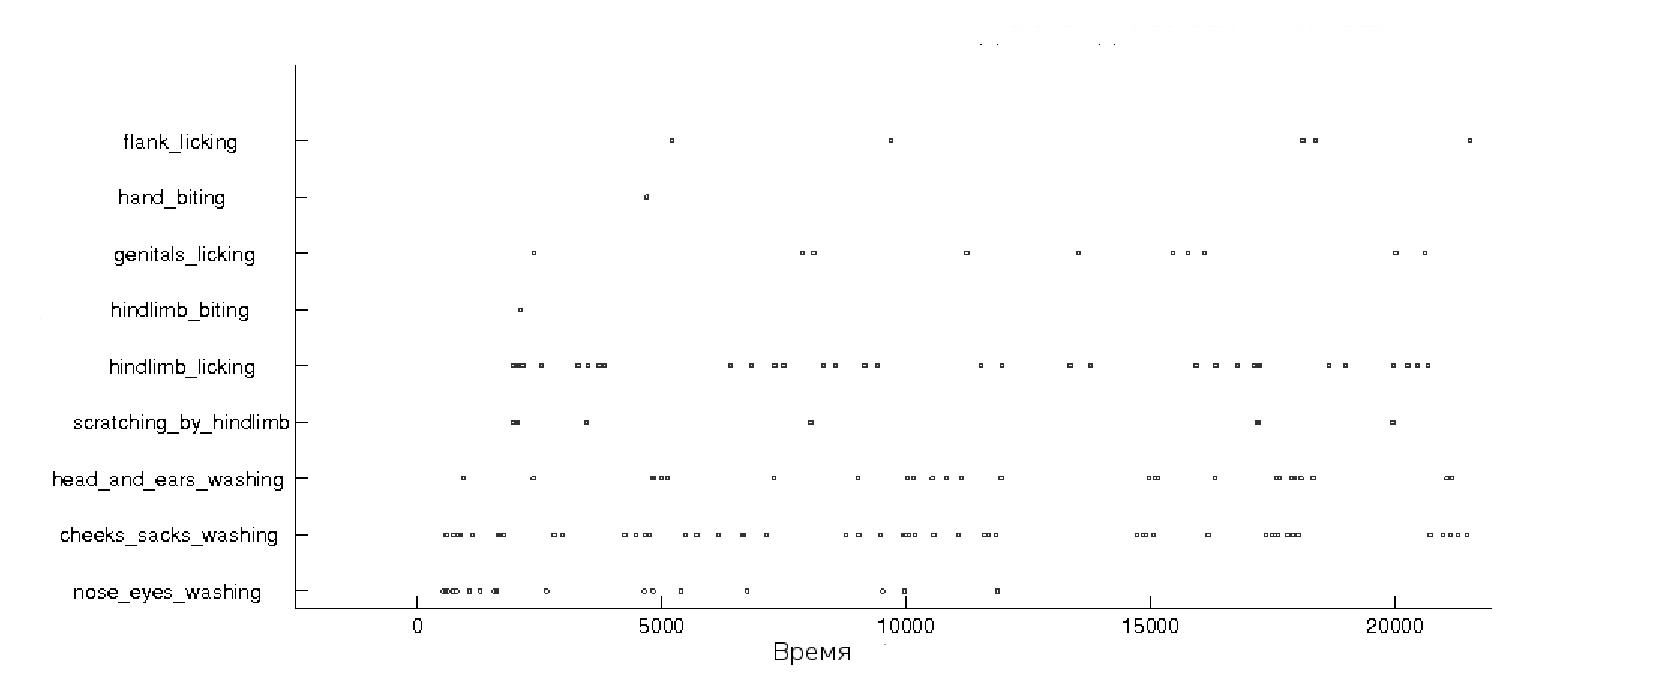
\includegraphics[width=163mm]{TS.eps}}
\caption{Пример реальных поведенческих данных. }
\end{figure}

Приведенные выше рассуждения дают понятие о том, что такое поведенческий паттерн, как его можно моделировать формальными терминами
(более точно определение Т-Паттерна(T-Pattern), введенное Магнусом Магнуссоном, дано в~\cite{Magnusson} ).
Иерархичная структура паттерна задает основы стратегии поиска подобных паттернов.

\subsection{ Определения и обозначения } \label{sec:defs}
Пусть время наблюдения разбито на $N_t$ интервалов. В каждый момент {\itshape периода наблюдения} $[\,1,N_t]$ 
может произойти некоторое событие $\evt$({\itshape действие, поведенческий акт, event}) 
\footnote{ Чаще всего понимается, что в этот момент времени имеет место {\itshape начало} действия} 
из множества допустимых событий $\mathcal{E}$ ({\itshape event types}). Соответственно, каждому типу события сопоставляется множество моментов 
времени $TS(\evt)$:
$$
TS(\evt) = \{ t^{\evt}_1,\dots, t^{\evt}_{N_{\evt} } \}, 
\qquad \evt\in\mathcal{E},\qquad
0\leqslant t^{\evt}_i \leqslant N_t,~~(i=1,\dots,N_t),
$$
здесь $N_{\evt}$~--- количество появлений события $\evt$ в данных.

Нечетким паттерном(далее P-Pattern, или просто паттерн)  $\pat$ длины $N_{\pat}$ назовем упорядоченную последовательность событий $\evt_i, (i=1,\dots N_{\pat})$, 
где каждое событие паттерна характеризуется смещением и разбросом от предыдущего события. Будем записывать паттерн
$\pat$ в следующем виде:
$$ \pat=\evt_1[\,\mu_1,\sigma_1]\evt_2[\,\mu_2,\sigma_2]\dots\evt_{N_{\pat}}[\,\mu_{N_{\pat}},\sigma_{N_{\pat}}], \qquad \mu_1=0. $$

Здесь $\mu_i$ и $\sigma_i$~--- смещение и разброс соответствующего события относительно предыдущего(см. Рис.~\ref{fig:ppttern}). 
Распределение межточечных расстояний~\cite[c.~138]{Shurygin} между событиями в паттерне моделируется нормальным распределением. 
Если нам не важны параметры смещения разброса событий, то паттерн записываться так: $\pat=\evt_1\evt_2\dots\evt_{N_{\pat}}$,
если нам важна иерархия паттерна, то например так: $\pat=((\evt_1\evt_2)(\evt_3\evt_4))$ 


\begin{figure}[H]
\noindent\centering{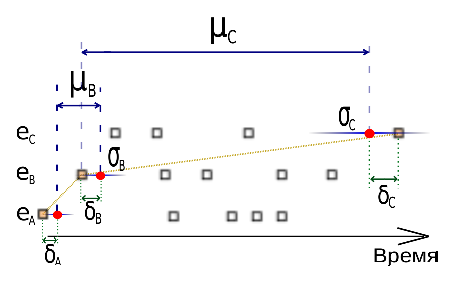
\includegraphics[width=113mm]{il1.eps}}
\caption{Представление нечеткого паттерна $ \pat=\evt_A[\,\mu_A,\sigma_A]\evt_B[\,\mu_B,\sigma_B]\evt_C[\,\mu_C,\sigma_C]$. }
\label{fig:ppttern}
\end{figure}

Далее, чтобы иметь возможность обрабатывать пропуски в реализации паттернов, 
введем понятие {\em функции потерь}, которая определяет <<штраф>> за пропуск
 $m$ событий в паттерне длины $N_{\pat}$ следующим образом:
$$
f_{LOSS}(m,N)= \begin{cases}
   \exp\left(-\frac{\lambda m}{N_{\pat}}\right), & m < N, \\
   0,                                    & m=N.
   \end{cases}
$$
Здесь $\lambda$ является структурным параметром, определяющим максимальный допустимый уровень
<<нечеткости>> паттернов. Если этот параметр велик, то мы, по сути, запрещаем реализациям
паттерна иметь пропуски. Если выставить этот параметр слишком малым, то будут обнаруживаться
паттерны, не разу полностью не встречающиеся в данных, то есть закономерности могут быть  найдены
даже в случайных данных. Данный параметр должен выставляться вручную, исходя из априорной информации
о типе данных, уровне шума, и сложности поведения. 

\begin{figure}[H]
\noindent\centering{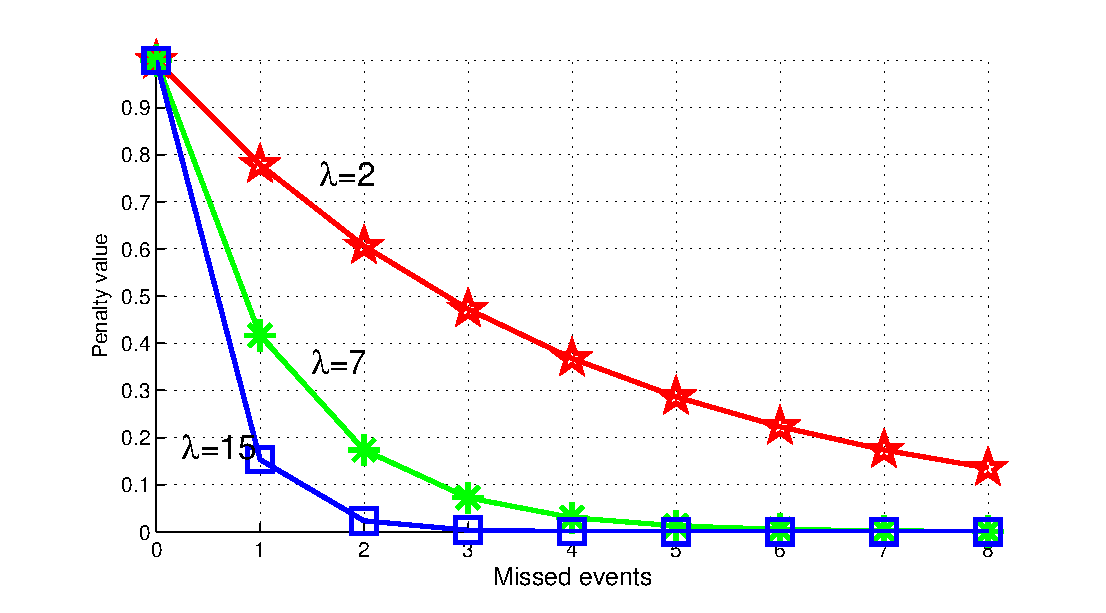
\includegraphics[width=123mm]{MB_LF.eps}}
\caption{ Функция потерь для паттерна длины 8 при разных значениях параметра $\lambda$. }
\end{figure}
%!!!!!!!!!!!!!!!!!!!!!!!!!!!!!!!!!!!!!!!!!!!!!!!!
%\newpage
\begin{figure}[H]
\noindent\centering{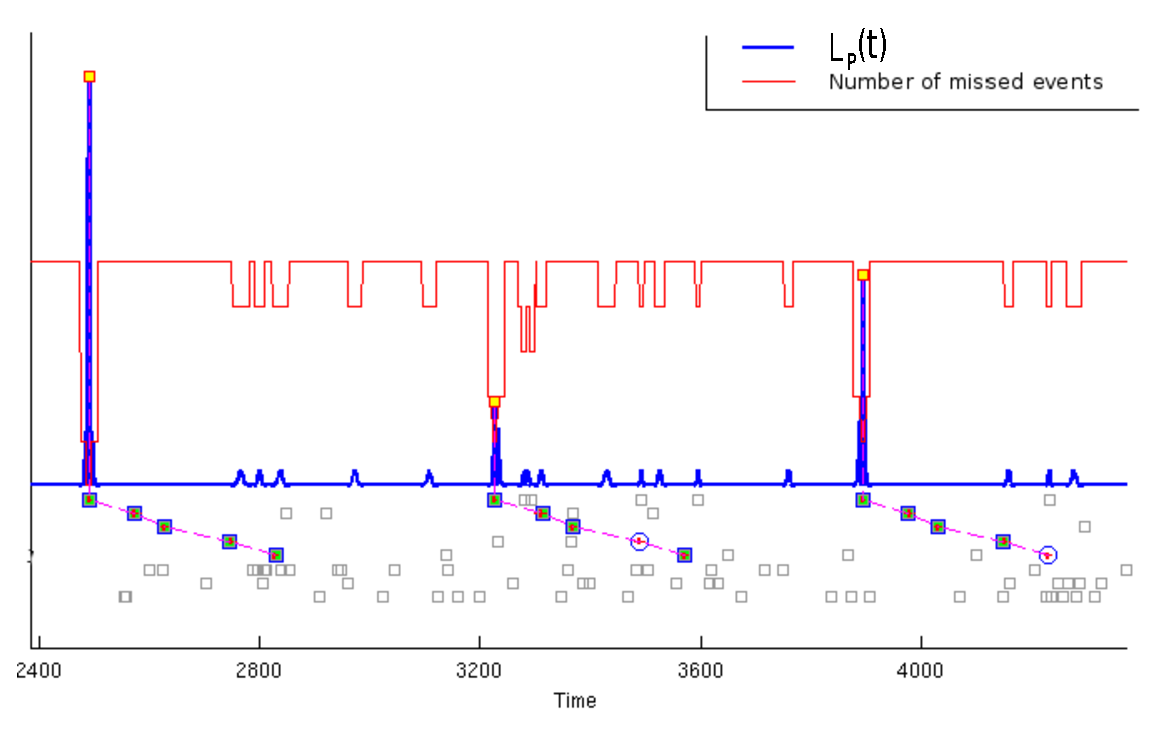
\includegraphics[width=163mm]{norm_12_of_14.eps}}
\caption{ Пример функции правдоподобия паттерна. Желтыми маркерами с красной границей изображены максимумы функции правдоподобия: 
моменты времени, когда мы считаем, что паттерн имеет место. Значение функции правдоподобия в максимуме будет весом $\alpha_{\pat,k}$
$k$-го появления паттерна $\pat$ в данных.
В нижней части рисунка закрашенными квадратами показаны присутствующие
события, полыми кружками~--- пропущенные события в паттерне. Полые серые квадраты соответствуют наблюдаемым поведенческим актам.}
\end{figure}
Теперь мы можем определить ключевое понятие для представленного метода~--- 
{\em правдоподобие паттерна}. Правдоподобие паттерна $\pat$~--- это функция, определенная
для каждого момента времени наблюдения $\varepsilon \: (\varepsilon=1,\dots, N_t)$, показывающая
на сколько четко можно говорить, что данный паттерн начинается в данный момент времени~$\varepsilon$. 
Более формально:
\begin{equation}\label{LHOOD}
L_{\pat}(\varepsilon)=
f_{LOSS}(N_-,N_{\pat})
\prod_{i=1}^{N_{\pat}}\left( \frac1{\sqrt{2\pi}\,\sigma_i }\right) 
\prod_{i\in \mathcal{N}_+}\exp\left(- \frac{\delta_i^2}{2\sigma_i^2}\right),
\end{equation}
здесь $\delta_i$~--- расстояния от ожидаемой позиции события в паттерне до ближайшего события в данных(более наглядно см. Рис.~\ref{fig:ppttern}). Т.е.:
$$
\delta_i=\min_{x\,\in\, TS(\evt_i)} \left|  
 \underbrace{\varepsilon+ \sum_{j=1}^{i-1}(\mu_j+\delta_j) + \mu_i}_{\text{ожидаемая позиция события}} -\, x
\right|,
$$
здесь, если событие было пропущено, то соответствующее $\delta_i=0$.
Далее, $N_-$~--- количество пропущенных событий в паттерне, а $\mathcal{N}_+$~--- множество индексов присутствующих в паттерне событий. Событие
считается пропущенным, если 
$\exp\left(- \frac{\delta_i^2}{2\sigma_i^2}\right)<\exp\left(-\frac{\lambda}{N_{\pat}}\right)$, т.е.
соответствующее значение $\delta_i$ больше определенного предела.



Заметим, что правдоподобие паттерна можно считать не только начиная с первого события, но и, например, с конца паттерна. Для упрощения вычислений,
значение правдоподобия паттерна $\pat$ с события $m$ можно рассчитывать по следующей формуле:
$$
L_{P,m}(\varepsilon)=L_P\left(\varepsilon+\sum_{j=1}^m\mu_j\right).
$$ 

На рисунке~\ref{fig:lhshift} видно, что правдоподобие, посчитанное с $m$-го события имеет максимумы в момент наступления $m$-го события
в текущем паттерне. Данный факт будет активно использоваться при вычислении межточечных расстояний между паттернами и в процессе
редукции паттернов-дубликатов.

\begin{figure}[!b]
  \begin{center}
   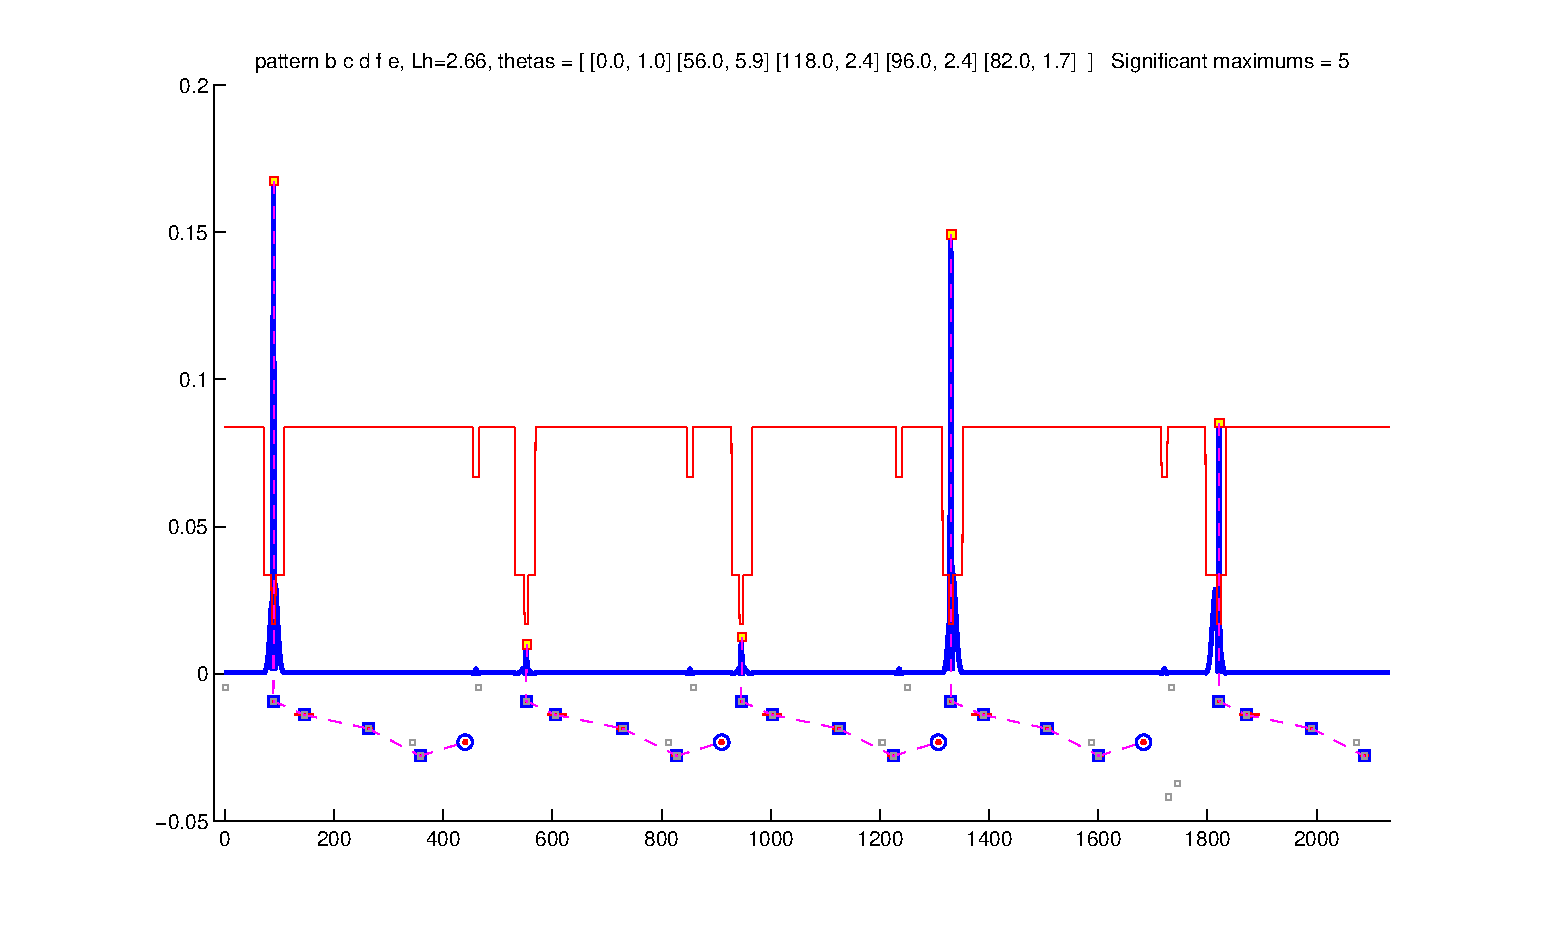
\includegraphics[width=143mm]{pat1.eps}
   \\
   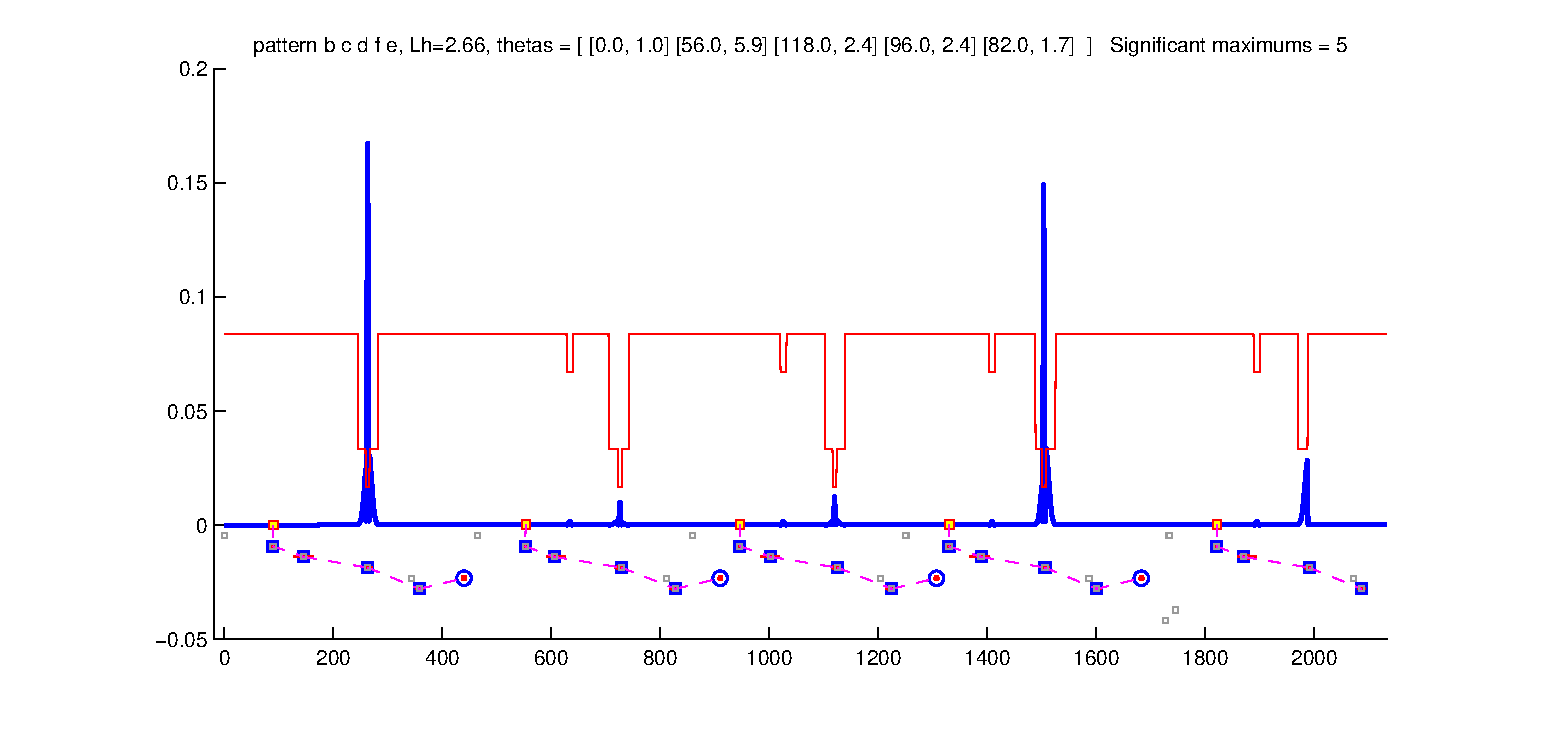
\includegraphics[width=143mm]{pat2.eps}
   \end{center}
\caption{Функция правдоподобия одного и того же паттерна, подсчитанная, начина с первого события $m=1$(сверху) и с
третьего события $m=3$(снизу).}
\label{fig:lhshift}
\end{figure}

\subsection{ Обзор существующих методов поиска паттернов и закономерностей }
Несмотря на то, что описанные выше паттерны широко распространены в описании поведения,
стандартные статистические методы не подходят для их поиска~\cite{Magnusson}. Еще сложнее 
приспособить статистические программные пакеты для выявления таких закономерностей.
Отчасти это объясняется тем, что для исследования более простых систем(не обязательно биологических), например, мух дрозофил,
достаточно оперировать более простыми статистическими данными о поведении. Закономерности в поведении таких систем можно моделировать, например,
с помощью периодических орбит из теории символьной динамики~\cite{POrbits}, в таком случае паттерн определяется только последовательностью
событий, но не временными интервалами, связывающими их. Так как поведение дрозофил достаточно примитивно(оно слабо варьируется, сильно предопределено
внешними факторами и предыдущими состояниями), описание возникающих паттернов периодическими орбитами вполне уместно~\cite{Stoop}. 
Однако для исследования поведения млекопитающих и, тем более, поведения человека, такие простые техники не могут описать
в требуемом объеме всю сложность поведения. И именно временн\'oе описание паттерна призвано решить проблему представления
и поиска поведенческих закономерностей в сложных системах.

Существует подход к поиску закономерностей в дискретных временных рядах, основанный
на проходе по исходных данных окном заданной ширины и подсчетом определенных частотных
характеристик в этом окне(например~\cite{PPE}). Но такой подход так же не удовлетворяет
поставленным требованиям к искомым закономерностям.

Методы поиска закономерностей из смежных областей, 
как правило, нацелены на поиск совершенно других структур: это либо просто определенные тренды во временных рядах, 
либо ассоциативные правила, которые не передают временн\'{у}ю и иерархическую структуру закономерности. Подход 
к поиску паттернов в активности нейронных культур~\cite{NS_1, NS_2}, в виду того, что приходится оперировать с 
крайне большими объемами данных, основывается на определении метрики между группами событий
и дальнейшей их кластеризации, также не подходит в случае анализа поведения животных. 

\subsection{Алгоритм поиска Т-Паттернов}
На сегодняшний день, для анализа временн\'{ы}х поведенческих закономерностей
наиболее широкое распространение получил метод поиска Т-Паттернов, предложенный в 2000-ом году
Магнусом Магнуссоном в~\cite{Magnusson}(также см. в~\cite{coursework}). Так как предложенный в нашей работе метод
является, по сути, расширением метода Магнуссона, опишем далее основные понятия алгоритма поиска Т-Паттернов.

Понятие паттерна вводится так же как, и в подразделе~\ref{sec:defs}, за исключением того, что каждое событие паттерна 
определяется фиксированным временн\'{ы}м интервалом, в течение которого это событие должно присутствовать
после предыдущего события. Другими словами, здесь расстояния между событиями моделируются не нормальным распределением,
а равномерным. Т-Паттерн обычно обозначается следующим образом:
$$\pat=\evt_1[\,d^1_L, d^1_R]\evt_2[\,d^2_L, d^2_R]\dots \evt_{N_{\pat}-1} [\,d^{N_{\pat}-1}_L, d^{N_{\pat}-1}_R] \evt_{N_{\pat}}.$$
Здесь запись $\evt_A[\,d_L, d_R]\evt_B$ обозначает, что событие $\evt_B$ должно присутствовать 
во временн\'{о}м интервале $[\,d_L, d_R]$ после события $\evt_A$, чаще, чем это ожидается при предположении 
о независимости событий. Более точно, при помощи биномиальной схемы, считается вероятность
текущей конфигурации распределения событий, принимая гипотезу, о том, что вероятность встретить событие 
$\evt$ в какой-либо момент времени равна $\frac{N_{\evt}}{N_t}$. Если эта вероятность меньше заданного
порога $\alpha$(обычно берется меньше $0.05$), то гипотеза о независимом равномерном распределении
событий отвергается и мы говорим, что $\evt_A[\,d_L, d_R]\evt_B$~--- Т-Паттерн, соединенный отношением
критической связи(critical relation). 
Точно такие же рассуждения
можно провести, взяв вместо событий $\evt_A$ и $\evt_B$ составные Т-Паттерны $\pat_A$ и $\pat_B$. Потребуется
только считать вхождения начала Т-Паттерна $\pat_B$ в интервале $[\,d_L, d_R]$ после конца Т-Паттерна $\pat_A$. 

\begin{figure}[H]
\noindent\centering{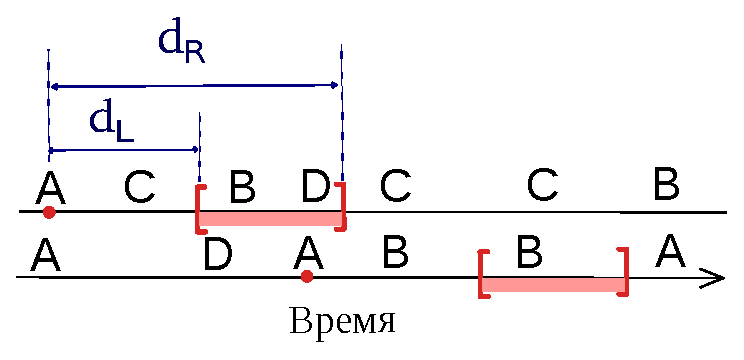
\includegraphics[width=83mm]{TPTSn.eps}}
\caption{ Отношение критического интервала $[\,d_1, d_2]$ между событиями $A$ и $B$. }
\end{figure}

Опишем этап {\em конструирования} Т-Паттернов: для всех пар Т-Паттернов, определяем, 
существует ли интервал $[\,d_L, d_R]$, связывающий эту пару паттернов критическим отношением. 
Если такой интервал существует, то мы добавляем новый Т-Паттерн. Если таких интервалов несколько,
то предлагается взять самый длинный интервал.

Для очистки множества найденных паттернов от паттернов-дубликатов и неполных копий существующих паттернов,
вводится процедура {\em редукции} множества Т-Паттернов: Т-Паттерн ${\bf Q_x}$ считается менее полным, чем ${\bf Q_y}$, 
если ${\bf Q_x}$ и ${\bf Q_y}$ появляются одинаково часто, и все события
возникающие в ${\bf Q_x}$, также возникают в ${\bf Q_y}$. Все Т-Паттерны попарно проверяются на полноту,
и если один паттерн признан менее полным, то он удаляется из текущего множества Т-Паттернов.

Предложенный алгоритм поиска заключается в итеративном повторении процедуры конструирования и процедуры редукции 
Т-Паттернов, пока текущее множество Т-Паттернов не перестанет изменяться. 

Несмотря на то, что алгоритм поиска Т-Паттернов и его программная
реализация в виде пакета \verb!THEME! хорошо зарекомендовали себя в исследовательских кругах, данный 
метод обладает рядом недостатков. Во-первых, само определение Т-Паттерна не позволяет паттерну иметь 
пропуски событий. Из-за этого метод становится крайне чувствителен к шуму в исходных данных, из-за чего
можно пропустить крайне информативные длинные и сложные паттерны. Во-вторых, процедура редукции
может оставить в текущем множестве два разны Т-Паттерна, являющихся одним и тем же поведенческим паттерном, если 
критические интервалы Т-Паттернов не совпадают. В-третьих, реализация данного алгоритма существует только
в дорогостоящем программном обеспечении от \verb!Noldus!, не позволяющем менять некоторые параметры поиска паттернов.

\section{Метод поиска нечетких паттернов}
Как упоминалось выше, предложенный метод основывается на алгоритме, предложенном в~\cite{Magnusson}. Основной целью 
являлось улучшение результатов работы алгоритма на зашумленных данных. Для этого в подразделе~\ref{sec:defs} описан модифицированный вид оригинальных Т-Паттернов,
названный P-Паттерном(probabilistic pattern), позволяющим поведенческим закономерностям  иметь пропущенные акты. Основой алгоритма будет 
аналогичная процедура итеративного повторения шагов конструирования и редукции паттернов. Но сами шаги 
конструирования и редукции, претерпели изменения, определенные тем, что было модифицировано само понятия паттерна.

\subsection{Поиск <<значимых>> максимумов функции правдоподобия}
Определенная выше функция правдоподобия P-Паттерна имеет много локальным максимумов, однако при визуальном рассмотрении,
обычно видно несколько ярко выраженных максимумов, в точках, которые можно считать началом вхождения паттерна.На шаге 
поиска новых закономерностей нам придется иметь дело с конкретными моментами времени, в которых имело место начало
паттерна. Поэтому требуется определить, какие именно точки максимумов действительно соответствую началам паттернов. 

Предположим, что в определенный момент времени $\varepsilon$ имело место начала модельного P-Паттрена(без пропусков событий) длины $N_{\pat}$. 
Запишем функцию правдоподобия:
$$
  L_{\pat}(\varepsilon)=\prod_{i=1}^{N_{\pat}}\frac1{\sqrt{2\pi}\,\sigma_i}\exp\left(-\frac{\delta_i}{2\sigma_i^2}\right),
  \quad\text{причем}\; \delta_j\sim\mathcal{N}(\,0,\sigma_j),\;(j=1,\dots,N_{\pat}).
$$ 
При таких условиях вычислим математическое ожидание $L_{\pat}(\varepsilon)$:
$$
\begin{aligned}
\mathbb{E}\left[L_{\pat}(\varepsilon)\right] &= \int\limits_{-\infty}^{+\infty}\!\dots\!\int\limits_{-\infty}^{+\infty}
L_{\pat}(\varepsilon) 
\prod_{i=1}^{N_{\pat}}\frac1{\sqrt{2\pi}\,\sigma_i}\exp\left(-\frac{\delta_i}{2\sigma_i^2}\right)
\, d\delta_1\dots d\delta_{N_{\pat}} =\\
&=\frac1{(2\pi)^{N_{\pat}}\prod_{i=1}^{N_{\pat}}\sigma_i^2}\: 
\prod_{i=1}^{N_{\pat}} \; \int\limits_{-\infty}^{+\infty}\exp\left( -\frac{\delta_i^2}{\sigma_i^2} \right)\,d\delta_i
=\frac1{(2\sqrt\pi\,)^{N_{\pat}}\,\sigma_1\dots\sigma_{N_{\pat}}}.
\end{aligned}
$$

Таким образом, нами получено характеристическое значение правдоподобия P-Паттерна длины $N_{\pat}$ с
параметрами разброса $\sigma_1,\dots,\sigma_{N_{\pat}}$. После чего, при поиске <<значимых>> максимумов 
отсекаются все локальные максимумы, значение которых меньше $\gamma\,\mathbb{E}\left[L_{\pat}(\varepsilon)\right]$,
где $\gamma$~--- заданное число от $0$ до $1$, в наших экспериментах обычно подходит значение $\gamma=0.4$. Если 
среди оставшихся максимумов есть точки, которые удалены друг на друга меньше длины паттерна, то берется
наибольший из них. Этот шаг объясняется тем, что один P-Паттерн не может иметь место в один и тот же момент времени.

\subsection{Процедура конструирования P-Паттернов}
Рассмотрим два P-Паттерна $\pat_L$(левый) и $\pat_R$(правый). Пусть $\{\alpha_i\}_{i=1,\dots,N_L}$ и $\{\beta_j\}_{j=1,\dots,N_R}$
~--- значения в <<значимых>> максимумах функций правдоподобия $L_{\pat_L}^{(end)}$ и $L_{\pat_R}$ соответственно. Заметим, что 
правдоподобие левого паттерна отсчитывается с конца, так как мы ищем связь между концом левого паттерна и началом правого.
Также пусть,  $\{x_{L,i}\}_{i=1,\dots,N_L}$ и $\{x_{R,j}\}_{j=1,\dots,N_R}$~--- индексы этих <<значимых>> максимумов. $N_L$ и
$N_R$~--- количество таких максимумов у паттернов $\pat_L$ и $\pat_R$ соответственно. Определим множество межточечных
расстояний:
$$
\rho=\{ x_{R,j}-x_{L,i}\: |\: x_{R,j} \geqslant x_{L,i}\}.
$$
Для каждого расстояния из этого множества введем соответствующий вес:
$$
w_l = \ln (1+\alpha_i\beta_j), \quad l=1,\dots,M,
$$
где $M=|\rho|.$

\begin{figure}[H]
\noindent\centering{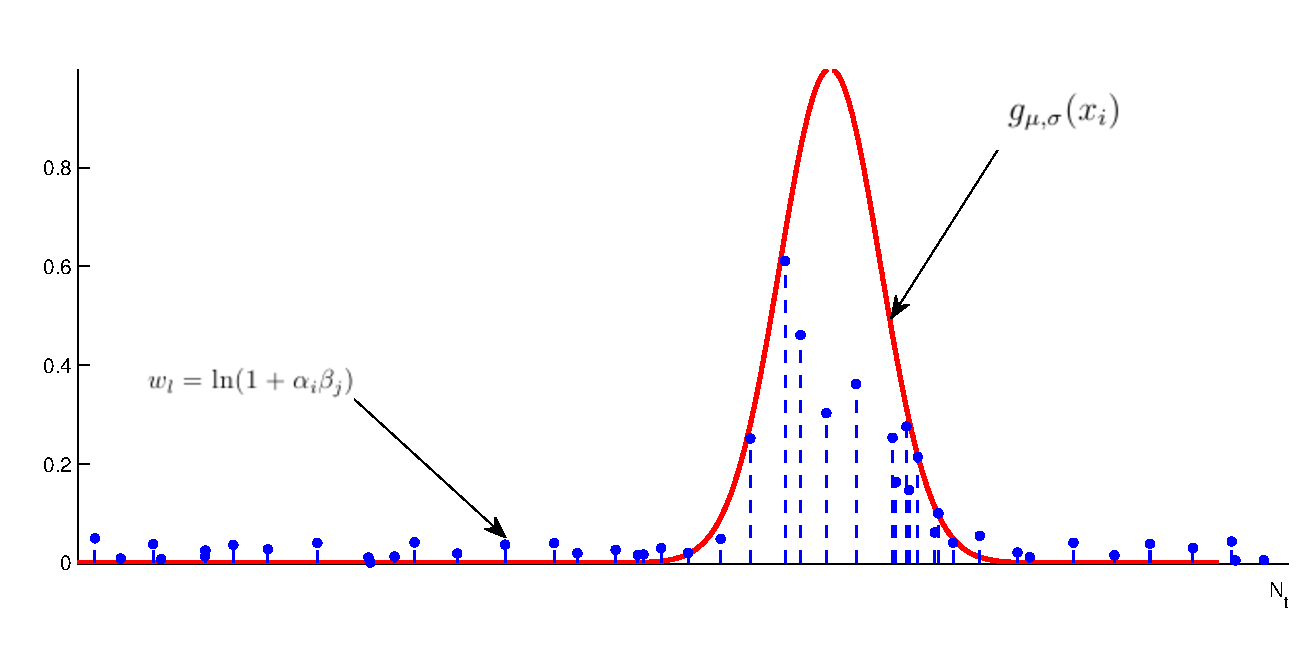
\includegraphics[width=153mm]{weights.eps}}
\caption{ Пример распределения межточечных расстояний и статистической модели связи.  }
\end{figure}


Примем гипотезу, что координаты <<значимых>> максимумов распределены независимо и 
равномерно на всем наблюдаемом промежутке, т.е. $x_{L,i}\sim\mathcal{U}[0,N_t], \quad x_{R,j}\sim\mathcal{U}[0,N_t]$. 
Тогда очевидно, что плотность распределение введенных выше межточечных расстояний имеет следующий вид:
$$
p(x_R-x_L\mid x_R \geqslant x_L ) = p_{LR}(x) =
\begin{cases}
  (N_t-x)\,\frac2{N_t^2} , & x \in [0,N_t], \\
  0, & x \not\in [0,N_t].
\end{cases} 
$$

Введем статистическую модель связи между паттернами(проверяемые параметры связи $\mu$ и $\sigma$ фиксированы):
$$
g_{\mu,\sigma}(x_i)=\frac{1}{\sqrt{2\pi}\,\sigma}\exp\left(- \frac{(x_i-\mu)^2}{2\sigma^2} \right).
$$
Рассмотрим следующую сумму:
\begin{equation}\label{k_stat}
k=\sum_{i=1}^M w_ig_{\mu,\sigma}(x_i)= \sum_{i=1}^M \xi_i, 
\end{equation}


где $x_i\sim p_{LR}$. О распределении значений $w_i$ мы не можем
делать никаких предположений, поэтому в вычислениях будем использовать выборочные моменты.

Для оценки распределения случайной величины $k$ проведем требуемые вычисления.
$$
\begin{aligned}
\mathbb{E} \left[ g_{\mu,\sigma} \right] &= \int\limits_{0}^{N_t}g_{\mu,\sigma}(x)\,p_{LR}(x)\,dx=
\int\limits_{0}^{N_t}g_{\mu,\sigma}(x)\,(N_t-x)\,\frac{2}{N_t^2}\,dx \approx \\
&\approx \frac2{N_t} \, \frac1{\sqrt{2\pi}\,\sigma}  \int\limits_{-\infty}^{+\infty}\exp\left( -\frac{(x-\mu)^2}{2\sigma^2} \right) \, dx 
- \frac2{N_t^2} \, \frac1{\sqrt{2\pi}\,\sigma} \int\limits_{-\infty}^{+\infty}x\,\exp\left( -\frac{(x-\mu)^2}{2\sigma^2} \right) \, dx = \\
&=\frac2{N_t} \left(1-\frac{\mu}{N_t}\right).
\end{aligned}
$$
$$
\begin{aligned}
\mathbb{E} \left[ g^2_{\mu,\sigma} \right] &= \int\limits_{0}^{N_t}g^2_{\mu,\sigma}(x)\,p_{LR}(x)\,dx=
\int\limits_{0}^{N_t}g^2_{\mu,\sigma}(x)\,(N_t-x)\,\frac{2}{N_t^2}\,dx \approx \\
&\approx \frac2{N_t} \, \frac1{2\pi\sigma^2}  \int\limits_{-\infty}^{+\infty}\exp\left( -\frac{(x-\mu)^2}{\sigma^2} \right) \, dx 
- \frac2{N_t^2} \, \frac1{2\pi\sigma^2} \int\limits_{-\infty}^{+\infty}x\,\exp\left( -\frac{(x-\mu)^2}{\sigma^2} \right) \, dx = \\
&=\frac1{N_t\sqrt{\pi}\,\sigma} \left(1-\frac{\mu}{N_t}\right).
\end{aligned}
$$
$$
\Var \left[ g_{\mu,\sigma} \right] = \mathbb{E} \left[ g^2_{\mu,\sigma} \right]  - \left( \mathbb{E} \left[ g_{\mu,\sigma} \right] \right)^ 2 = 
\left( 1-\frac{\mu}{N_t} \right)\,\left( \frac1{{N_t}\sqrt{\pi}\,\sigma} - \frac{\mu}{{N_t}^2} \left( 1- \frac{\mu}{N_t} \right) \right).
$$
Далее считаем параметры случайной величины $\xi_i=w_ig_{\mu,\sigma}(x_i)$. Здесь $\overline{w}$ и $\hat{w}$~--- выборочное среднее и дисперсия весов, соответственно.
$$
\mathbb{E}\left[ \xi_i \right] = \mathbb{E}\left[ w g_{\mu,\sigma}(x) \right] = 
\mathbb{E}\left[ w_i\right]    \mathbb{E}\left[  g_{\mu,\sigma}(x_i) \right] \approx \overline{w} \: \frac2{N_t} \left(1-\frac{\mu}{N_t}\right).
$$
Запишем  дисперсию произведения независимых случайных величин:
$$
\Var \left[ \xi_i \right] = \Var \left[ w\, g_{\mu,\sigma} \right] = 
\left( \mathbb{E}\left[ g_{\mu,\sigma} \right]\right)^2 \hat{w} +
\Var\left[ g_{\mu,\sigma} \right] \overline{w}^2 + \hat{w}\, \Var\left[ g_{\mu,\sigma} \right].
$$
Тогда по Центральной Предельной Теореме:
$$
\begin{aligned}
&\sum_{i=1}^M \xi_i\!=\!k\: \sim\: \mathcal{N}\left(\mu_\ast, \sigma_\ast^2 \right), \:\text{где} \\
&\mu_\ast= M\,  \mathbb{E} \left[ \xi_i \right], \\
&\sigma_\ast^2 =  M \, \Var \left[ \xi_i \right].
\end{aligned}
$$

Теперь можно провести сравнение подсчитанного на реальных данных значения $k$ с 
правым односторонним квантилем уровня $\alpha$. 
Если односторонняя гипотеза о равномерном распределении событий с моделью связи $g_{\mu,\sigma}$ 
отвергается, то из паттернов $\pat_L=\evt^L_1[\,\mu^L_1,\sigma^L_1]\dots\evt^L_{N_{\pat_L}}[\,\mu^L_{N_{\pat_L}},\sigma^L_{N_{\pat_L}}]$ и 
$\pat_R=\evt^R_1[\,\mu^R_1,\sigma^R_1]\dots\evt^R_{N_{\pat_R}}[\,\mu^R_{N_{\pat_R}},\sigma^R_{N_{\pat_R}}]$ конструируется новый
паттерн длины $N_L+N_R$:
$$
\pat=\evt^L_1[\,\mu^L_1,\sigma^L_1]\dots\evt^L_{N_{\pat_L}}[\,\mu^L_{N_{\pat_L}},\sigma^L_{N_{\pat_L}}]
\:\evt^R_1[\,\mu,\sigma]\dots\evt^R_{N_{\pat_R}}[\,\mu^R_{N_{\pat_R}},\sigma^R_{N_{\pat_R}}].
$$
Если существует несколько пар $\mu$ и $\sigma$, для которых отвергается гипотеза, то для конструирования P-Паттернов берутся
непересекающиеся\footnote{$[\,\mu'-3\sigma', \mu'+3\sigma']\cap[\,\mu''-3\sigma'', \mu''+3\sigma'']=\varnothing$} параметры
соответствующие максимальным значениям $k$.

Отметим, что замена пределов интегрирования(для $\mathbb{E} \left[ g_{\mu,\sigma} \right]$ и
$\mathbb{E} \left[ g^2_{\mu,\sigma} \right]$) с 0 до $N_t$ на всю прямую, дает плохой результат, когда
$\mu$ близко к $N_t$. Данный случай не критичен при поиске поведенческих закономерностей, так как на практике 
обычно не требуется искать такие длинные связи:
даже если они будут найдены, то этот паттерн будет состоять не более, чем из двух элементов. 
Однако при проверке таких пар $\mu$ и $\sigma$ можно вычислять точное значение интеграла через функцию ошибок:
$$
\begin{aligned}
\mathbb{E} \left[ g_{\mu,\sigma} \right] =& \int\limits_{0}^{N_t}g_{\mu,\sigma}(x)\,(N_t-x)\,\frac{2}{N_t^2}\,dx = \\
=& \frac{\mu-N_t}{N^2_t} \left[  \Erf\left( \frac{\mu-N_t}{\sqrt{2}\,\sigma}\right) - \Erf\left( \frac{\mu}{\sqrt{2}\,\sigma}\right)  \right] +\\
&+\frac1{N_t^2}\exp\left(-\frac{\mu^2+N_t^2}{2\sigma^2}\right)\sqrt{\frac2\pi}\,\sigma\left( 
\exp\left(\frac{\mu N_t}{\sigma^2}\right)-\exp\left(\frac{N^2_t}{2\sigma^2}\right)
\right),
\end{aligned}
$$
$$
\begin{aligned}
\mathbb{E} \left[ g^2_{\mu,\sigma} \right] =& \int\limits_{0}^{N_t}g^2_{\mu,\sigma}(x)\,(N_t-x)\,\frac{2}{N_t^2}\,dx = \\
=& \frac1{2\pi\sigma N^2_t} 
\Biggl[  
\sqrt\pi\,\left( \mu-N_t \right) \left( 
\Erf\left( \frac{\mu-N_t}{\sigma}\right) - \Erf\left( \frac\mu\sigma\right)  \right) +\\
+& \sigma \left( 
\exp\left(-\frac{(\mu-N_t)^2}{\sigma^2}\right) - \exp\left(-\frac{\mu^2}{\sigma^2}\right)
\right)
\Biggr].
\end{aligned}
$$

\subsection{Процедура редукции множества P-Паттернов}
Так же как и в методе Магнуссона, наш алгоритм может конструировать
P-Паттерны являющиеся дубликатами, или неполными копиями уже обнаруженных
P-Паттернов. Далее дадим более полное описание этой проблемы.
\begin{trivlist}
\item {\bf Паттерны-дубликаты}:
\\Один и тот же паттерн может быть сконструирован из разных подпаттернов. Например
P-Паттерн $\evt_A\evt_B\evt_C\evt_D$ может быть получен как путем соединения
паттернов $\evt_A\evt_B$ и $\evt_C\evt_D$, так и паттернов $\evt_A\evt_B\evt_C$ и $\evt_D$.
Обычно такие P-Паттерны представляют одну и ту же поведенческую закономерность,
но из-за сложного процесса соединения паттернов, функции правдоподобия
этих двух паттернов-дубликатов могут отличаться.

\item {\bf Неполные копии паттернов}:
\\Конструируя паттерны из подпаттернов, некоторые подпаттерны
могут появляться в данных только в составе более сложных составных
паттернов(см. Рис.~\ref{fig:duppat}. Такие подпаттерны не имеет смысла рассматривать отдельно, поэтому
их надо удалять из множества найденных P-Паттернов.
\end{trivlist}
\begin{figure}[H]
\noindent\centering{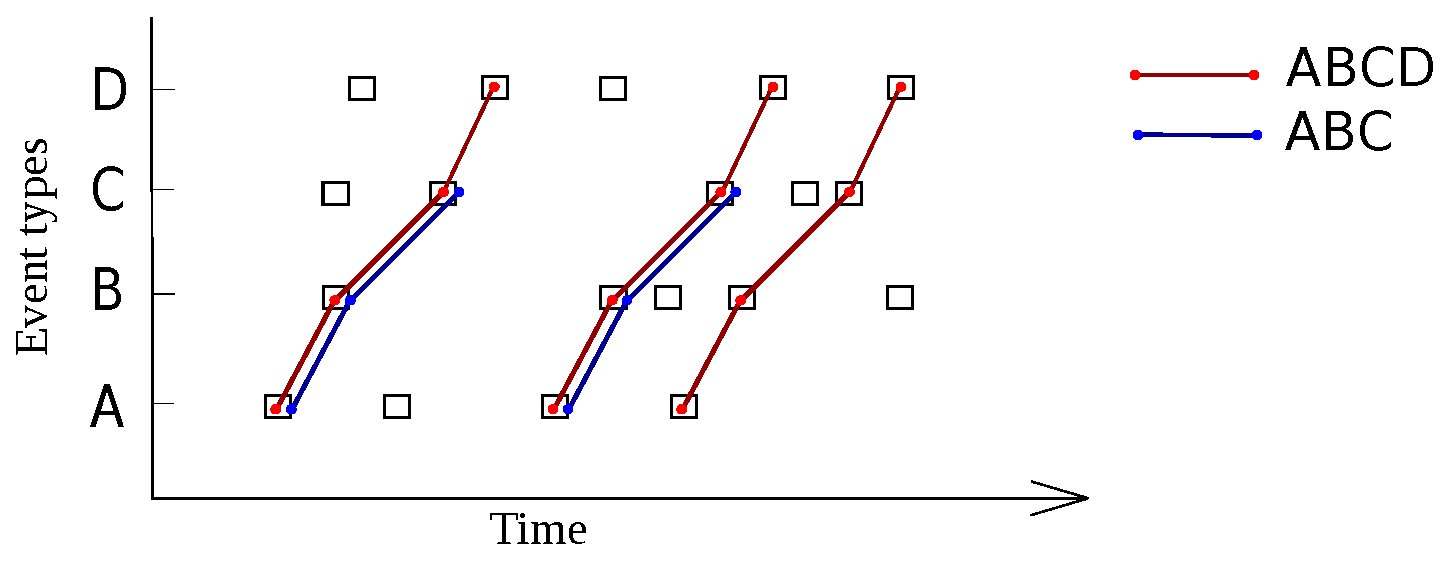
\includegraphics[width=133mm]{dup_2.eps}}
\caption{ Здесь $BCD$~--- неполная копия паттерна $ABCD$. Заметьте, что правдоподобия 
$ABCD$ и $BCD$ отсчитанное от первого события будут похожими.  }
\label{fig:duppat}
\end{figure}

Для удаления таких P-Паттернов предлагается анализировать
коэффициент корреляции функций правдоподобия. Пусть $\overrightarrow{L_{\pat,i}}$~---вектор-столбец
значений функции правдоподобия, отсчитанной от $i$-го события во всех моментах времени наблюдения.
$$
cor\left(\overrightarrow{L_1}, \overrightarrow{L_2}\right) = 
\frac{{\overrightarrow{L_1}}^\top \overrightarrow{L_2}}{ 
\sqrt{ {\overrightarrow{L_1}}^\top \overrightarrow{L_1} }\,\sqrt{ {\overrightarrow{L_2}}^\top \overrightarrow{L_2} } }
\:\in[\,0,1]
$$
~--- коэффициент корреляции между двумя P-Паттернами. Чем он ближе к $1$, тем два паттерна 
более близки друг к другу.

Процедура редукции паттернов выглядит следующим образом: перебираем все пары $\pat_L, \pat_R$
из множества найденных паттернов. Если все поведенческие акты, присутствующие в паттерне $\pat_L$ 
также присутствуют в $\pat_R$ с учетом порядка, и 
$$
\exists m\colon\: cor\left(\overrightarrow{L_{P_L,1}}, \overrightarrow{L_{P_R,m}} \right) > \nu,
$$
тогда паттерн $\pat_L$ удаляется из множества найденных паттернов. Отметим, что в данном методе
не удаляются псевдопаттерны(паттерны состоящие из одного события), так как они могут быть необходимы для конструирования закономерностей на
следующих шагах.

\subsection{Алгоритм поиска P-Паттернов} 
После описания основных шагов конструирования и редукции P-Паттернов, можно описать сам алгоритм
поиска:
\begin{enumerate}
 \item Инициализировать текущее множество паттернов псевдопаттернами.
 \item Для всевозможных пар паттернов из текущего множества для которых не было произведено попытки их слития, 
провести процедуру конструирования паттернов. Сконструированные паттерны, которые встречаются в данных не менее 
$N_{min}$ раз, добавить в текущее множество.
 \item Для всевозможных пар паттернов из текущего множества, провести процедуру редукции паттернов.
 \item Если текущее множество паттернов изменилось, перейти к п.2.
\end{enumerate}

Очевидно, что описанный выше метод остановится, так как на каждом шаге будут
произведены попытки сконструировать паттерны все б\'{о}льшей длины, а одни и те же паттерны
не проверяются больше одного раза.

Предложенный в данной работе алгоритм обладает рядом параметров, которые не настраиваются 
автоматически. Эти параметры должны быть выставлены вручную исследователями, исходя из
априорных сведений о типе исходных данных, или ожидаемого вида поведенческих закономерностей. 
Список этих структурных параметров с объяснениями и значениями по-умолчания представлен в 
Таблицу~\ref{tab:pars}.

\begin{table}
\begin{tabular}{|p{5em} | p{7em} | p{7em} | p{14em}| }
    \hline
    \bf{Параметр} & \bf{ Возможные\newline значения} & \bf{ Значения по-умолчанию} &\bf{ На что влияет } \\
    \hline\hline
    \centering$\alpha$   & \centering$[\,0, 1]$ & \centering $0.01$ & Уровень значимости паттерна \\ \hline
    \centering$N_{min}$ &  \centering$[\,0, +\infty]$ & \centering 3 & Минимальное количество появлений паттерна в данных  \\ \hline 
    \centering$\lambda$  & \centering$[\,0, +\infty]$ & \centering 8 & Допустимая степень нечеткости паттерна  \\  \hline    
    \centering$\nu$      & \centering$[\,0, 1]$ & \centering 0.6 & Минимальная степень похожести паттернов для удаления \\ \hline
    \centering$\gamma$   & \centering$[\,0, 1]$ & \centering 0.4 & Чувствительность к отклонению от ожидаемого правдоподобия \\ \hline
\end{tabular}
 \caption{Параметры алгоритма поиска P-Паттернов.}
\label{tab:pars}    
\end{table}

Отметим, что предложенный алгоритм является отчасти переборным, а самыми вычислительно-сложными 
процедурами являются подсчет функции правдоподобия для каждого паттерна, отсчитанная для каждого события, и
подбор параметров смещения и разброса при попытке конструирования паттернов. Для ускорения работы,
была реализованная параллельная версия данных процедур, описанная в подразделе~\ref{sec:ppat_parallel}. 

\subsection{Случайные паттерны}
Когда исследования проводятся на больших наборах данных, то закономерности могут возникать даже, если выборка была сгенерированна случайно. 
Поэтому, для найденного множества паттернов было бы полезно оценить, являются ли они случайными, или <<структурными>>. 
Одним из подходов к решению данной задачи, является анализ рандомизированных данных:
\\
для каждого массива данных создаются данные с такой же протяженностью периода наблюдения и 
мощностью множества допустимых событий, но для каждого допустимого события
 $\evt_i$, моменты времени его появления генерируются случайно из равномерного на $[\,0, N_t]$ распределения с вероятностью $N_{\evt_i}/N_t$.
Для полученных данных применяется процесс поиска паттернов с {\itshape теми же параметрами}, которые применялись на исходных данных. 
Описанные действия исполняются несколько раз,
после чего результаты поиска на рандомизированных данных сравниваются с исходными. 

Считается, что поиск паттернов прошел успешно, если в исходных данных было выявлено значительно больше закономерностей, чем в рандомизированных, 
или они оказались длиннее~\cite{Magnusson}.

\section{Параллельная реализация методов поиска закономерностей}
Как было отмечено выше, рассмотренные алгоритмы поиска закономерностей
имеют переборную составляющую. Так как при более полном переборе вариантов, позволяющем находить
более длинные и значимые паттерны, время работы алгоритма увеличивается, то имеет смысл произвести распараллеливание метода.
В общем случае,
при полном переборе всевозможных Т-Паттернов, алгоритм имеет экспоненциальную сложность от количества
возникших событий в данных(см. Рис.~\ref{fig:excomp}).
Возможны два подхода к параллельной реализации данного алгоритма. 
\begin{itemize}
\item 
Во-первых, можно разбивать каждую итерацию алгоритма на, очевидно,
независимые подзадачи сравнения пар паттернов(на шагах конструировании, редукции паттернов, и
вычислении правдоподобия каждого паттерна). В этом случае, подзадачи вообще не требуют пересылки
данных между собой, кроме как для инициализации и возвращения результата работы. Получается, что
мы, фактически, одновременно обрабатываем несколько паттернов на разных вычислительных узлах. Такой 
подход можно реализовать на современных многоядерных системах с общей памятью(symmetric multiprocessing),
или на вычислительных кластерах. 
\item 
Во-вторых, можно распараллеливать саму процедуру конструирования и 
вычисления правдоподобия паттернов. Тогда все паттерны будут обрабатывать последовательно, друг за другом,
но очень быстро из-за того, что проверка реализована параллельно. Такой подход не может быть эффективно реализован,
на вычислительном кластере, из-за большого количества пересылок данных между вычислительными узлами. Возможно более
эффективная реализация для многоядерной архитектуры, но так как исходная задача разбивается на крайне простые 
подзадачи, то самым уместным решением будет использование современных программируемых графических чипов, 
работающих по схеме SIMD(Single Instruction Multiple Data). 
\end{itemize}
\begin{figure}[H]
\noindent\centering{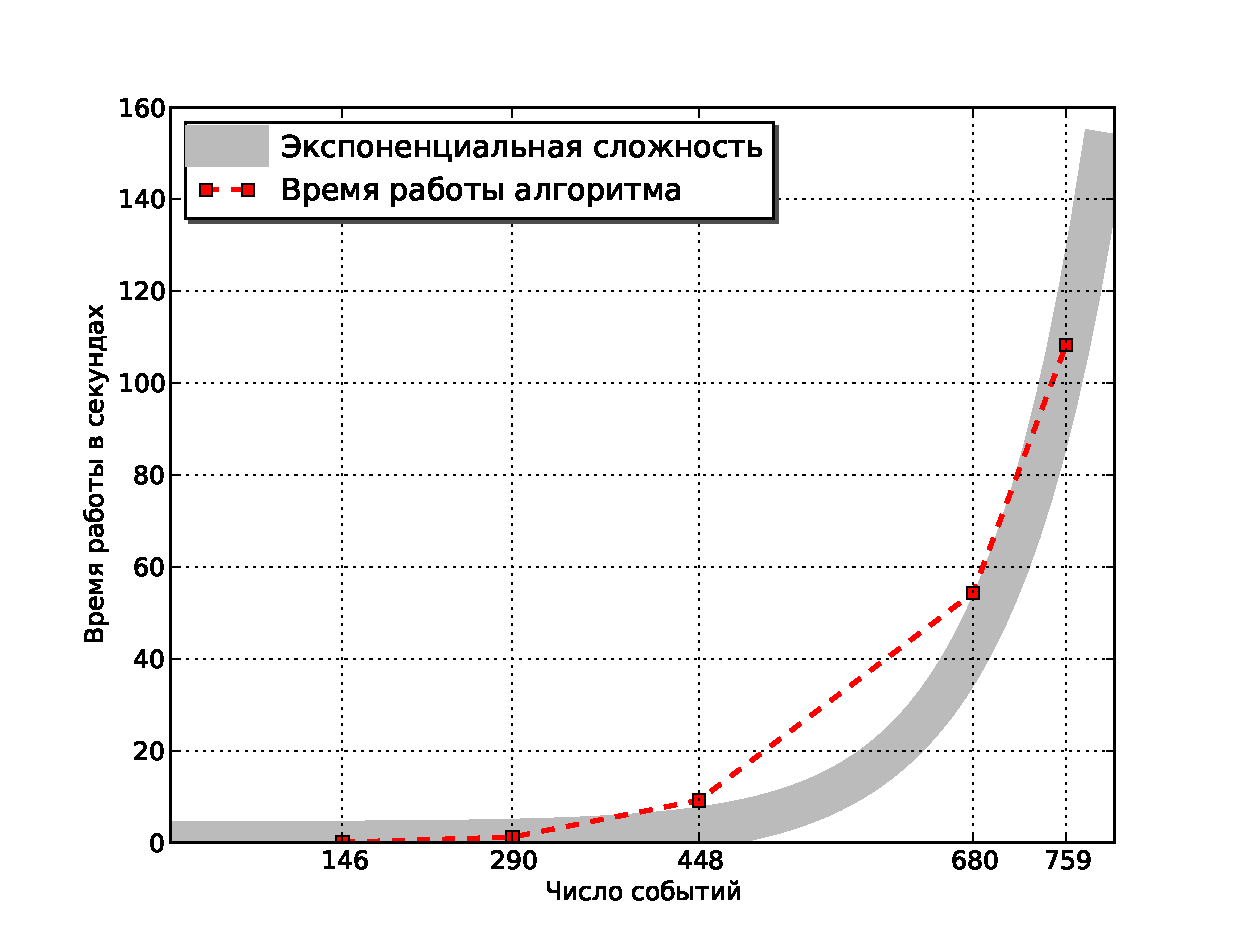
\includegraphics[width=133mm]{tp_comp.eps}}
\caption{ Сложность алгоритма поиска Т-Паттернов в зависимости от количества событий в данных.  }
\label{fig:excomp}
\end{figure}

\subsection[Параллельная реализация алгоритма поиска T-Паттернов]{Параллельная реализация алгоритма поиска <<четких>> закономерностей(Т-Паттерны)}
Для параллельной реализации метода поиска Т-Паттернов, предложенного Магнуссоном, мы
первый подход, где алгоритм разбивается на подзадачи обработки паттернов. Последовательная
версия алгоритма была реализована нами ранее на языке \verb!C!, поэтому мы произвели 
распараллеливание метода для архитектуры SMP с помощью \verb!OpenMP!. 

Результаты полученного ускорения представлены на графике~\ref{fig:omp_tp} и в Таблице~\ref{tab:omp_tpt} Техническая 
реализация была достаточна тривиальна: этапы конструирования и редукции Т-Паттернов были 
помещены в параллельную секцию с описанием локальных и общих участков памяти, после чего на каждом
шаге проводится сбор результатов работы со всех вычислительных узлов и модификация текущего множества найденных Т-Паттернов.
Распределение подзадач по вычислительным узлам производит встроенный в \verb!OpenMP! планировщик, простой
вычислительных узлов возможен, только в конце каждой итерации алгоритма, когда не остается необработанных пар паттернов.

\begin{figure}[H]
	\begin{multicols}{2}
	\hfill
	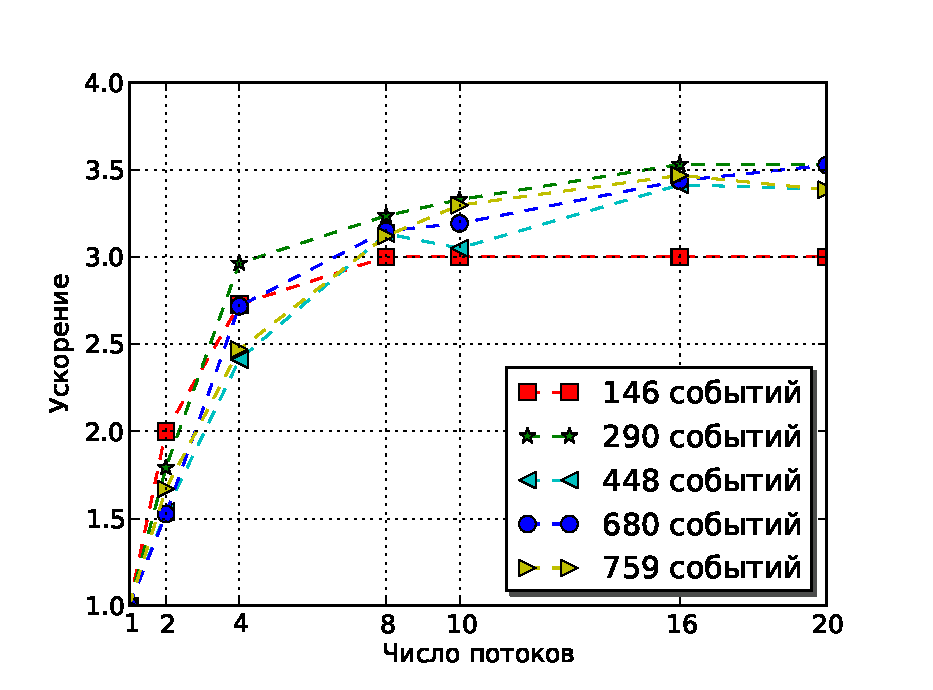
\includegraphics[width=90mm]{omp_su.eps}

	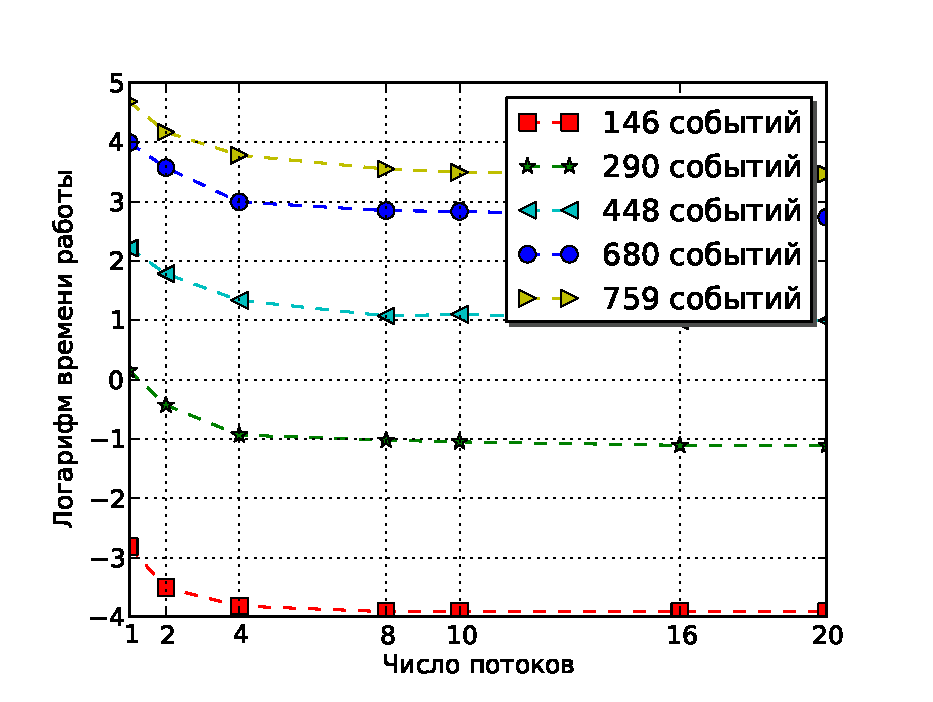
\includegraphics[width=90mm]{omp_t.eps}
	\end{multicols}
	\caption[Параллельная реализация алгоритма поиска T-Паттернов]{Время работы и ускорение алгоритма поиска Т-Паттернов на 4-х ядерном процессоре.}
\label{fig:omp_tp}
\end{figure}

На большинстве примеров видно, что увеличение количества потоков
ожидаемо уменьшает время работы программы. Как и стоило ожидать, на задачах с большим количеством 
событий, мы получаем большее ускорение при большом количестве узлов. Так как эксперименты производились
на 4-х ядерном процессоре, то при количестве потоков большем, чем 4 ускорение перестает быть линейным.


\subsection[Параллельная реализация алгоритма поиска P-Паттернов]{Параллельная реализация алгоритма поиска <<нечетких>> закономерностей(P-Паттерны)}
\label{sec:ppat_parallel}
Алгоритм поиска P-Паттернов является еще более вычислительно-сложным, чем алгоритм поиска Т-Паттернов,
поэтому для его применения на реальных данных крайне важна параллельная реализация. 
Для распараллеливания алгоритма была использована технология \verb!NVIDIA CUDA!, позволяющая 
создавать программы, в том числе, для современных игровых видеокарт, которые широко распространены 
и имеют один из самых выгодных показателей FLOPS(FLoating point OPerations per Second) за доллар. 

Подробное описание архитектуры \verb!GPU! от \verb!NVIDIA! и технологии \verb!CUDA! можно найти,
например, в~\cite{NV_doc, Boreskov_CUDA}. Отметим лишь, что логически все вычисления на \verb!GPU!
разбиваются на блоки({\em blocks}), блоки, в свою очередь, разбиваются на нити(потоки, {\em threads}). 
Нити из одного блока могут синхронизироваться и обмениваться данными через высокоскоростную shared-память.
Нити из одного блока физически выполняются на одном мультипроцессоре {\em half-warp'}ами(группы по 16 нитей), 
что нужно учитывать при доступе к различным видам памяти. Также существуют доступные и крайне эффективные~\cite{Boreskov_CUDA, NV_reduction}
схемы одного из важнейших параллельных примитивов: параллельной редукции. Крайне важно избегать ветвлений 
внутри  {\em half-warp'}ов, так как мультипроцессор исполняет  одновременно одни и те же операции
для нескольких разных данных(схема SIMD).

При этом, между нитями на \verb!CPU! и нитями на \verb!GPU! есть принципиальные различия~\cite{Boreskov_CUDA}:
\begin{itemize}
\item нити на \verb!GPU! обладают крайне <<небольшой стоимостью>>~--- их создание и управление требует минимальных ресурсов (в отличии от \verb!CPU!);
\item для эффективной утилизации возможностей \verb!GPU! нужно использовать многие тысячи отдельных нитей (для \verb!CPU! обычно нужно не более 10-20 нитей)
\end{itemize}

В нашей реализации на \verb!GPU! были перенесены две самые вычислительно-сложные процедуры: конструирование паттернов, 
вычисление правдоподобия паттерна. Предложенная конкретная реализация проектировалась с учетом спецификаций
устройств \verb!NVIDIA Compute Capability 1.1!. Данная спецификация определяет, например, доступные инструкции чипа, 
объем типов памяти, количество регистров.

Для параллельной версии конструирования паттернов использовался следующий подход: разные блоки соответствуют
разным {\em парам} тестируемых параметров $\mu$ и $\sigma$ для двух паттернов. В shared-память каждого
блока загружается множество межточечных расстояний, после чего эффективным образом вычисляется статистика $k$~(\ref{k_stat})
для каждой данной пары параметров.  Данная статистика сравнивается с фиксированным порогом и принимается решение
о добавлении паттерна в текущее множество.

Для параллельной версии процедуры вычисления правдоподобия использовался следующий подход: моменты времени, в которых вычисляется
правдоподобие разбиваются на участки, соответствующие блокам, каждый участок, в свою очередь, состоит из моментов времени,
каждый из которых соответствует нити внутри блока. Далее, производится процесс редукции для поиска ближайшего элемента
паттерна и по формуле~(\ref{LHOOD}).

Вычислительные эксперименты(см. Рис.~\ref{fig:cuda_D},\ref{fig:cuda_L}) проводились на устройстве \verb!NVIDIA! \verb!GeForce 8800GTX! 
с 128 потоковыми процессорами, вычисления проводились с одинарной 
точностью(single precision floating-point format). Для процедуры конструирования паттернов удалось достичь ускорения работы в 15--20 раз, а для процедуры вычисления правдоподобия
было получено ускорение в 120--140 раз, что соответствует максимальному порядку ускорения задач для данной архитектуры~\cite{CUDA_showcase}. Общее ускорение
работы программы, в среднем, 40 раз. Например, при разметке поведения на 80 поведенческих актов($N_t=2401$), последовательная версия на используемом
оборудовании работает 423~сек., параллельная версия~--- 11~сек. 
Скорее всего, для современных \verb!GPU!(\verb!GeForce 8800GTX! был выпущен в 2006-ом году), имеющих большее количество потоковых процессоров и shared-памяти, возможно
создать еще более эффективную реализацию, которая будет проводить вычисления уже с двойной точностью(double precision floating-point format). 

\begin{figure}[H]
	\begin{multicols}{2}
	\hfill
	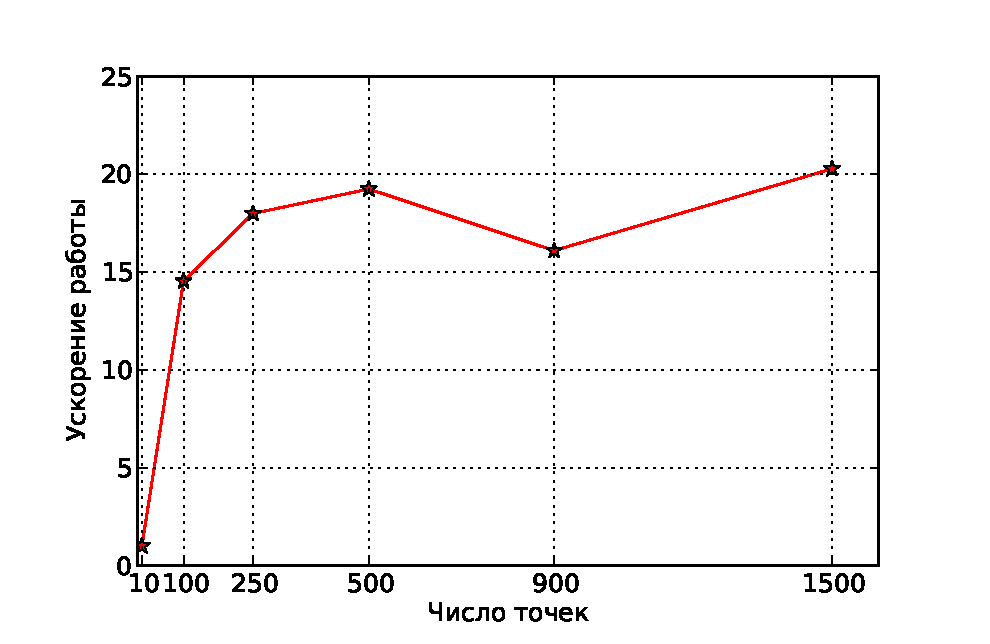
\includegraphics[width=90mm]{cuD_su.eps}

	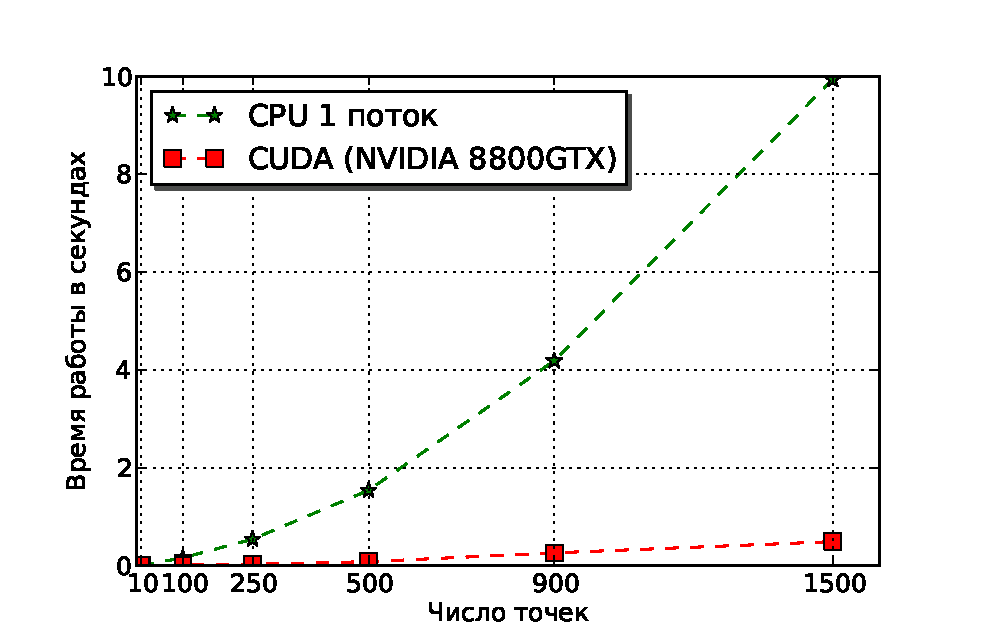
\includegraphics[width=90mm]{cuD_t.eps}
	\end{multicols}
	\caption{Время работы и ускорение процедуры конструирования P-Паттернов на GPU и CPU.}
\label{fig:cuda_D}
\end{figure}

\begin{figure}[H]
	\begin{multicols}{2}
	\hfill
	\includegraphics[width=90mm]{cuL_su.eps}

	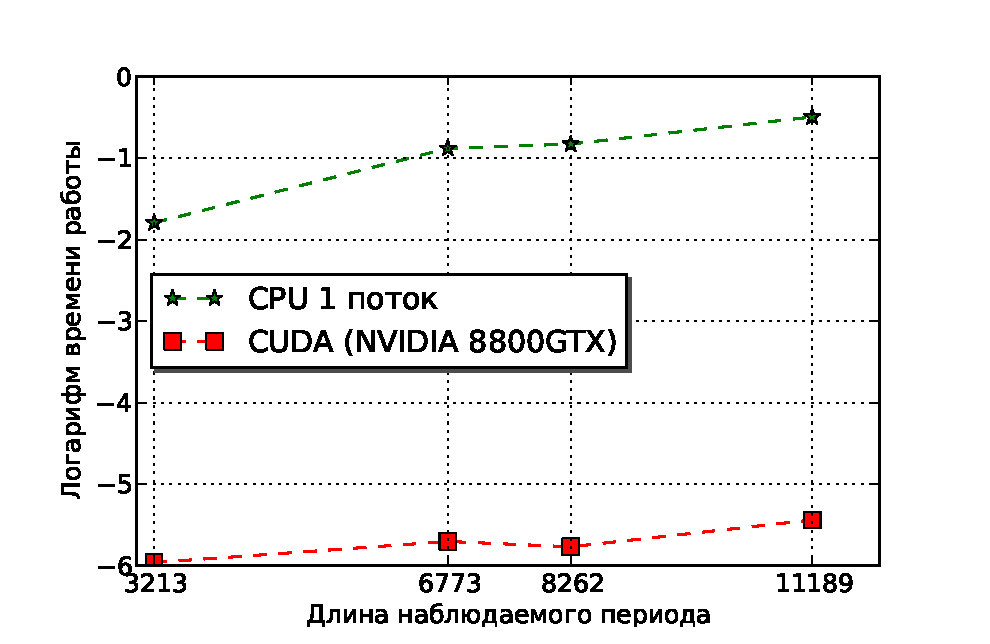
\includegraphics[width=90mm]{cuL_t.eps}
	\end{multicols}
	\caption{Время работы и ускорение вычисления правдоподобия P-Паттернов на GPU и CPU.}
\label{fig:cuda_L}
\end{figure}



\section[Сравнение методов. Результаты работы на реальных данных]{ Сравнение алгоритмов поиска Т-Паттернов и P-Паттернов. Результаты работы на экспериментальных данных}
\subsection{Сравнение результатов алгоритмов поиска Т-Паттернов и P-Паттернов }
Предложенный в данной работе алгоритм поиска P-Паттернов создавался, как расширение
исходного алгоритма поиска Т-Паттернов, поэтому логично требовать, чтобы паттерны найденные
исходным алгоритмом(по крайней мере самые длинные), также были найдены предложенным методом. Сложность заключается
в том, проблематично точно сопоставить найденный Т-Паттерн с найденным P-Паттерном. Данная работа была
сделана вручную. Результаты показывают, что среди P-Паттернов найденных предложенным методом, в среднем, присутствует более 90\%~\cite{MB_article} 
Т-Паттернов, найденных исходным методом(см. Рис.~\ref{fig:tp_fp_cmp}). Более того, предложенный метод находит более длинные закономерности(см. Рис.~\ref{fig:tp_fp_cmp}).
На модельных зашумленных данных, как и ожидалось, метод поиска P-Паттернов находит более длинные версии Т-Паттернов(пример на Рис.~\ref{fig:tp_fp_missed}).
\begin{figure}[H]
	\begin{multicols}{2}
	\hfill\vfill
	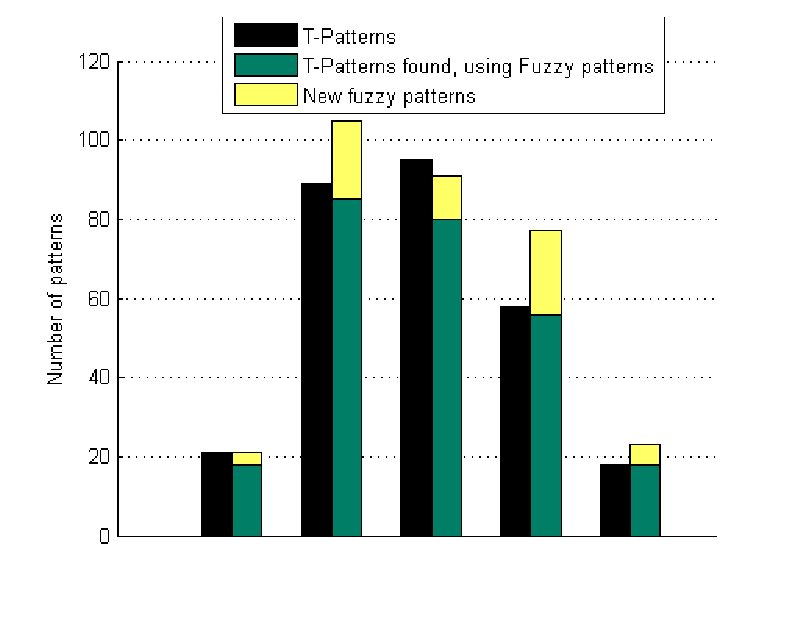
\includegraphics[width=90mm]{exx.eps}

	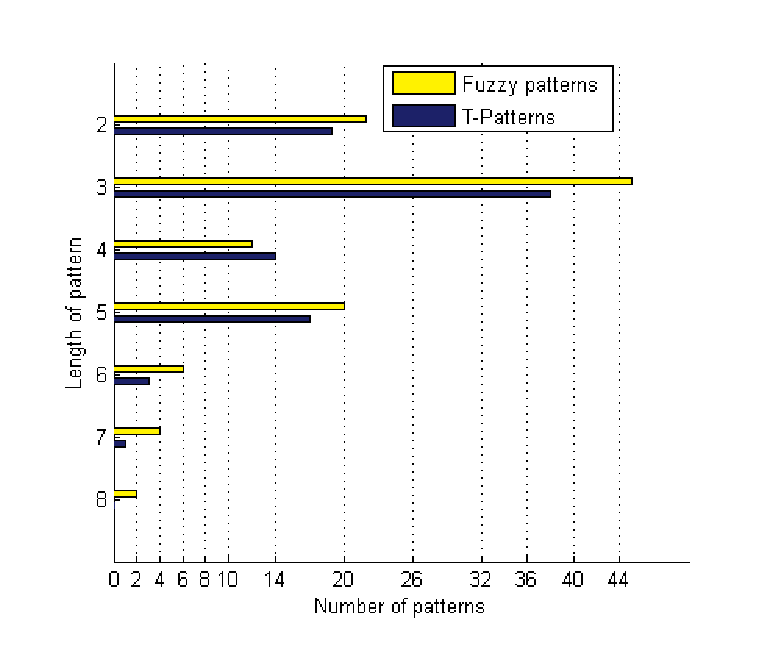
\includegraphics[width=90mm]{hist.eps}
	\end{multicols}
	\caption{Слева: количество паттернов, найденных разными методами. Справа: распределение длин найденных паттернов.}
\label{fig:tp_fp_cmp}
\end{figure}
\begin{figure}[H]
\noindent\centering{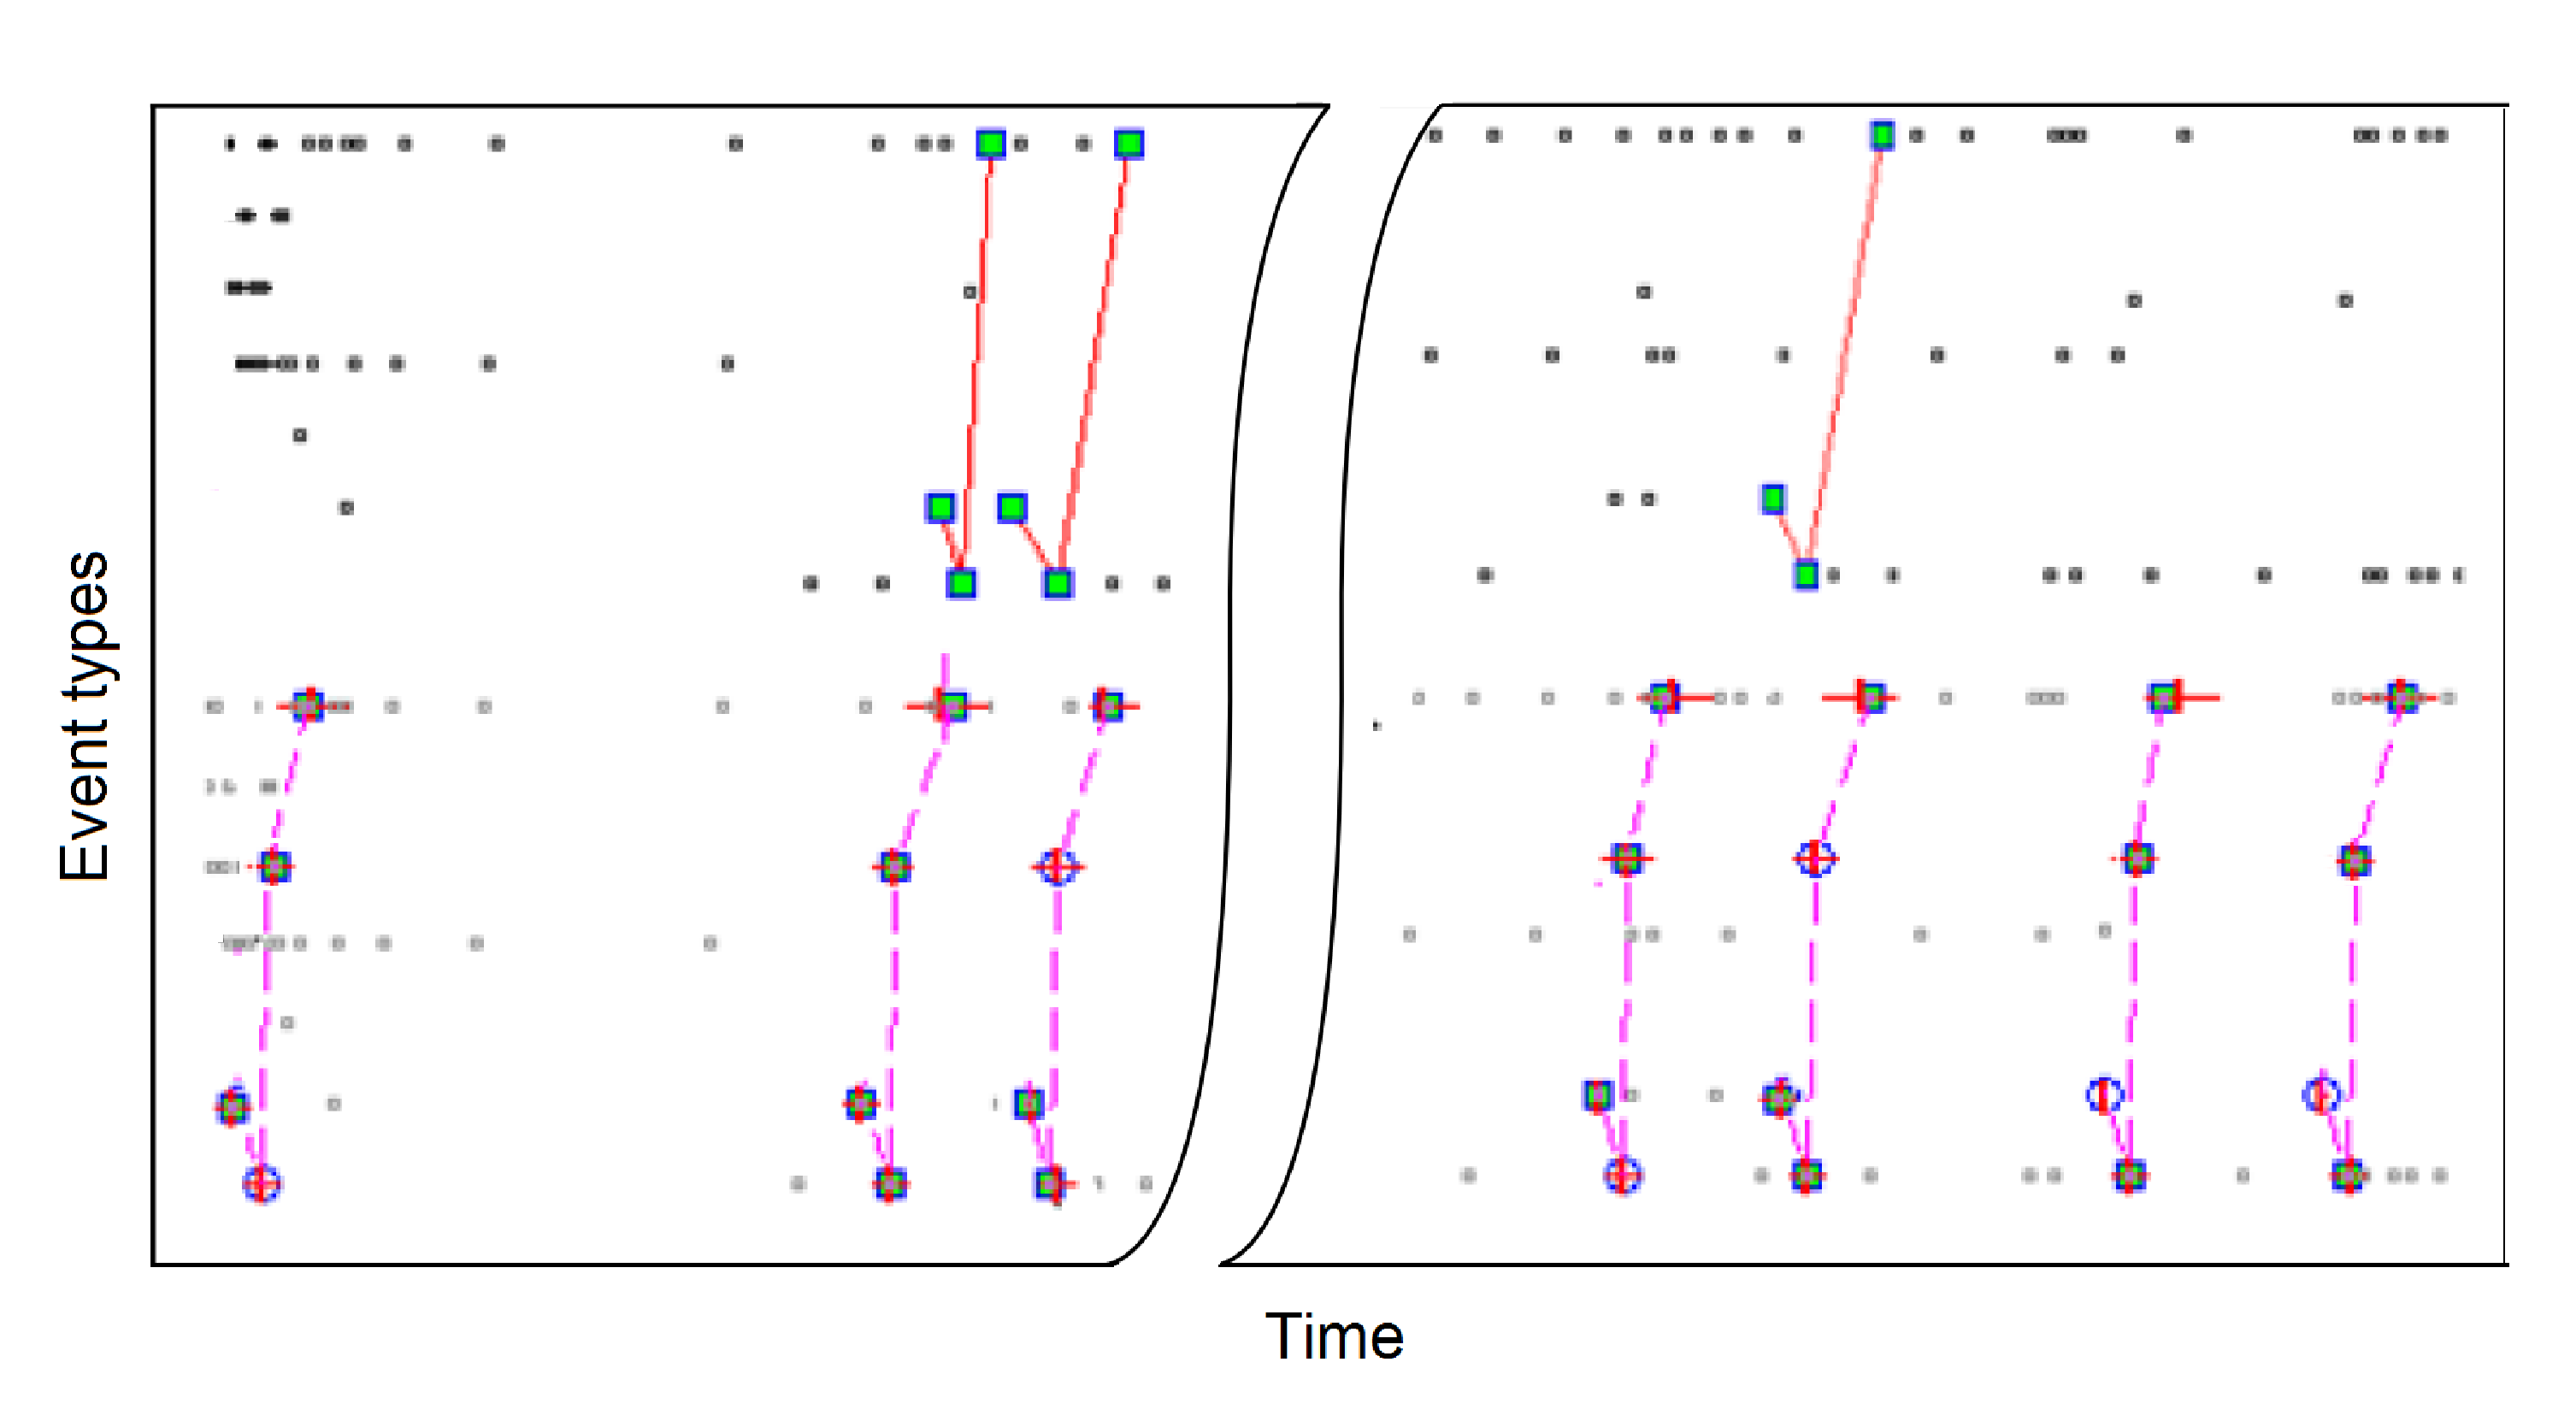
\includegraphics[width=153mm]{tsss.eps}}
\caption{ Сравнение найденных закономерностей в реальных данных, используя алгоритм поиска Т-Паттернов(сверху)
и алгоритм поиска P-Паттернов(снизу). Пропущенные события показаны полыми кружками. P-Паттерны имеют б\'{о}льшую длину
и чаще встречаются в данных. Этот объясняется тем, что в данных не присутствует достаточно экземпляров паттерна без пропусков. }
\label{fig:tp_fp_missed}
\end{figure}

\subsection{Эксперименты на реальных данных}
Описанный ниже эксперимент демонстрирует способ применения предложенного метода на реальных поведенческих
данных. Целью эксперимента является анализ того, как влияет отсутствие гиппокампа
на поведение. Гиппокамп~--- один из древнейших отделов головного мозга млекопитающих, его функции 
связывают с механизмами работы памяти(консолидация информации из краткосрочной в долгосрочную память), обучением, пространственной
навигацией~\cite[c.~744]{Neuro_exploring_the_brain}.

Мы располагали данными о поведении мелких мышеобразных грызунах~---~рыжих полевках. Исследуемые особи
разбиваются на две группы по 12 в каждой. Грызуны из первой группы(контрольной)~--- нормальные, здоровые особи,
грызуны из второй группы~--- гиппокамп данных животных разрушали путем введения в эту структуру лидокаина, растворенного в искусственной спинномозговой жидкости (2 мкл. 4\% 
раствора), лидокаин обладает местно-анестезирующим действием, блокирует потенциал-зависимые натриевые каналы, что препятствует генерации импульсов клетками. 
Используемая доза блокатора вызывала длительную инактивацию клеток структуры, что в дальнейшем приводило к их отмиранию и разрушению части структуры. Данные
видеонаблюдения за грумингом(процесс умывания, очистки поверхности тела животным) каждой отдельной
особи были размечены  на поведенческие акты, приведенные в Табл.~\ref{tab:grooming_acts}. 

Для каждой из 24-х особей был произведен поиск паттернов. Далее, для всех пар 
особей $(i,j)$ вычислялось число {\em соответствий}  паттернов, найденных 
у $i$-ой особи в поведении $j$-ой особи:
$$
match(i,j) = \sum_{\pat\in Patters(i)}[ N_{\pat} \geqslant MinPat ]\, c^\beta(\pat, j),
$$
где $Patterns(i)$~--- множество паттернов, найденное в поведении особи $i$, 
$N_{\pat}$~--- длина паттерна $\pat$,
$c(\pat, j)$~--- количество найденных вхождений паттерна $\pat$ в поведении
особи $j$, $[~]$~--- скобки Аверсона. Параметр $MinPat$ определяет минимальную длину паттернов, соответствия которых мы ищем, 
данный параметр имеет смысл ставить б\'{о}льшим, или равным 3, так как короткие паттерны
зачастую являются шумовыми. Параметр $\beta$ может принимать значения из $\mathbb{R}$,
однако самыми осмысленными являются значения 0 и 1. При $\beta=1$ число соответствий
между особями $i$ и $j$ равно сумме числа вхождений всех паттернов(длиннее чем $MinPat$) 
особи $i$ в поведении особи $j$. При $\beta=0$ число соответствий
между особями $i$ и $j$ равно количеству {\em разных паттернов} особи $i$, встречающихся
в поведении особи $j$. Отметим, что при $\beta=0$ число соответствий более инвариантно
к длине периода наблюдения за животным.
\begin{figure}[H]
\noindent\centering{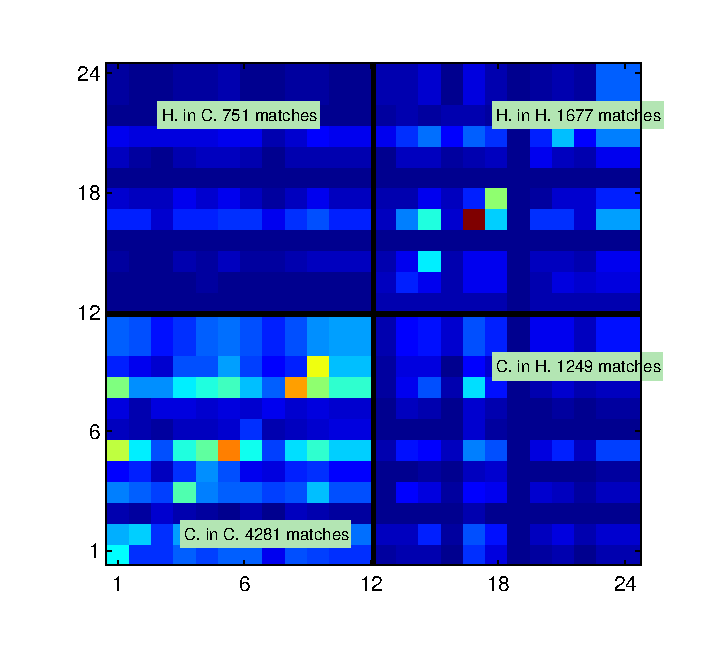
\includegraphics[width=93mm]{cross_m_big.eps}}
\caption{ Таблица соответствий $match(i,j)$ для $MinPat=4$, $\beta=0$. По вертикали отложены значения $i$, по горизонтали~--- $j$(неформально: 
по вертикали {\em откуда} берутся паттерны, по горизонтали~--- {\em где} ищутся вхождения этих паттернов; например, в ячейке $(3,10)$ записано
число соответствия паттернов третей особи в поведении десятой). Матрица, вообще говоря, не должна быть 
симметричной.}
\label{fig:cross}
\end{figure}
\begin{figure}[t]
\noindent\centering{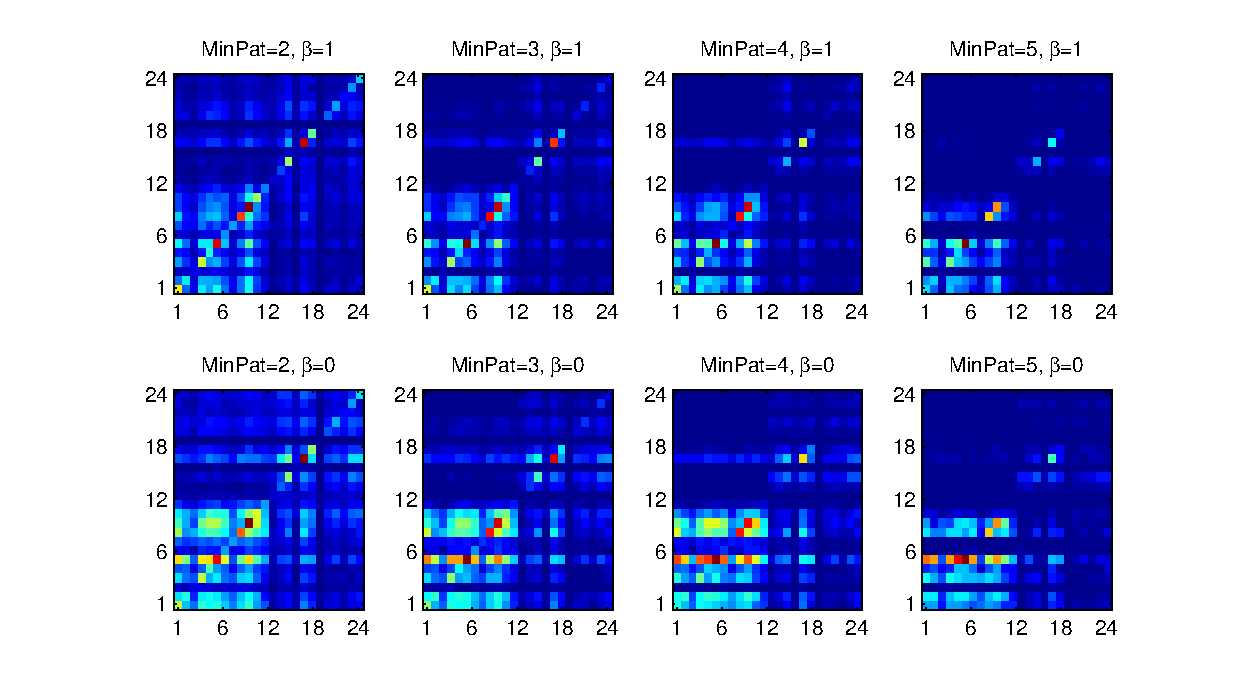
\includegraphics[width=173mm]{cross_m_diff.eps}}
\caption{ Разные способы подсчета числа соответствий.}
\label{fig:cross_many}
\end{figure}

На Рис.~\ref{fig:cross}\ref{fig:cross_many} видно, что исследуемые группы хорошо разделимы по введенной выше таблице соответствий. 

Используя таблицу соответствий паттернов можно провести классификацию особей. В задаче классификации объектом $\varphi_i$
возьмем вектор
  $$ \varphi_i = \left(\,match(i,1), \dots, match(i,N)\,\right), $$
здесь $N$~--- общее число особей(в нашем случае 24). Таким образом, объект, соответствующий особи $i$
является вектором <<откликов>> на паттерны $i$-ой особи в поведении других особей.

Мы рассмотрели два метода решения задачи классификации: метод опорных векторов(SVM),
метод $k$ ближайших соседей($k$NN). Также было проведено сравнение качества классификации, используя 
P-Паттерны и Т-Паттерны. Отметим, что в методе $k$ ближайших соседей упорядочивание соседей
проводилось не по Евклидовой метрике между введенными выше векторами, а по количеству 
соответствий($match(i,j)$) паттернов данного объекта $i$ с объектами из обучения $j$.

\begin{figure}[t]
\noindent\centering{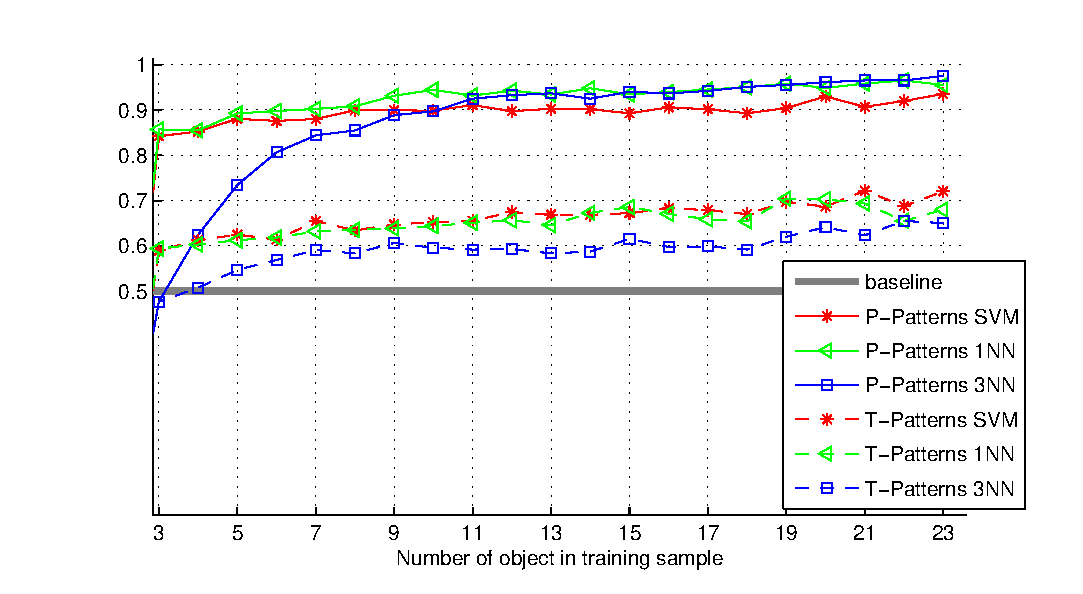
\includegraphics[width=173mm]{2classes.eps}}
\caption{ Средняя доля правильных ответов классификации методами SVM, 1NN, 3NN, с разными способами поиска паттернов, в зависимости от размера
обучающей выборки. Параметры подсчета числа соответствий: $MinPat=4, \; \beta=0$, данные значения были взяты для обеспечения <<чистоты>> эксперимента. }
\label{fig:class2}
\end{figure}

Анализируя Таб.~\ref{tab:2classes} и Рис.~\ref{fig:class2}, можно сделать следующие выводы:
\begin{itemize}
 
\item классификация при использовании метода поиска P-Паттернов производится на порядок
точнее, чем при использовании существующего метода поиска Т-Паттернов;
\item для классификации особей, используя P-Паттерны, можно использовать 
любой из рассмотренных методов классификации,  имея в виду, что метод $k$ ближайших соседей при $k=3$ имеет низкое качество классификации
на короткой обучающей выборке;
\item при классификации с использованием P-Паттернов доля правильных ответов, в среднем, равна 92\%.
\end{itemize}

Также, в качестве эксперимента, в исходные данные были добавлены еще 2 группы: рандомизированные данные
(события равномерно распределены по интервалу наблюдения) и данные с искусственными паттернами. Таблица соответствий
и качество классификации показано на Рис.~\ref{fig:4classes}. Таким образом, мы продемонстрировали, что:
\begin{itemize}
 \item 
 предложенным методом можно проводить классификацию на несколько классов; 
\item
группа особей с нарушением работы гиппокампа может быть отличена от рандомизированных 
данных, несмотря на то, что априорно, поведение таких особей <<проще>> и содержит
меньше паттернов.
\end{itemize}

\begin{figure}[!t]
	\begin{multicols}{2}
	\hfill
	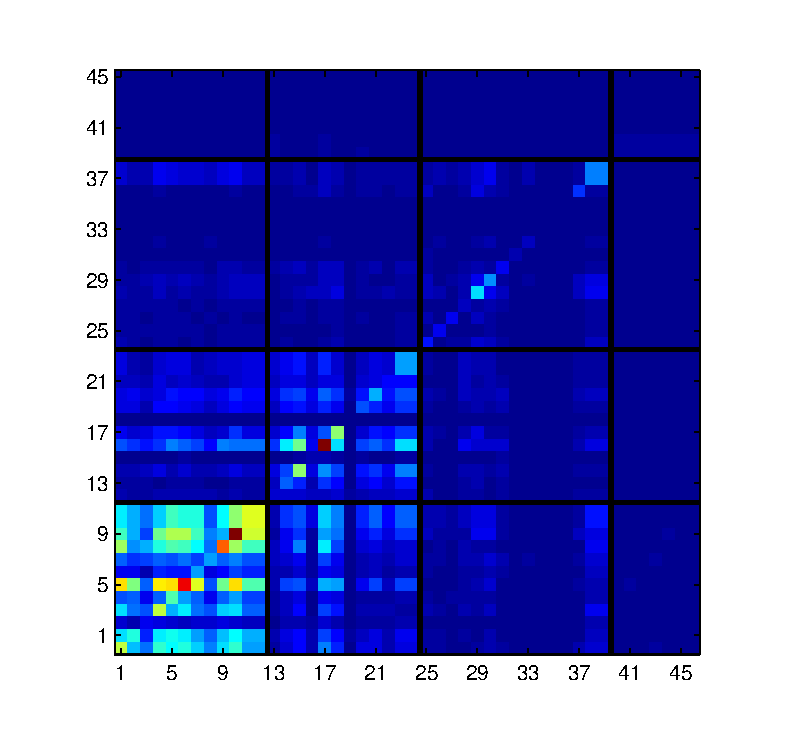
\includegraphics[width=90mm]{4classes_match.eps}

	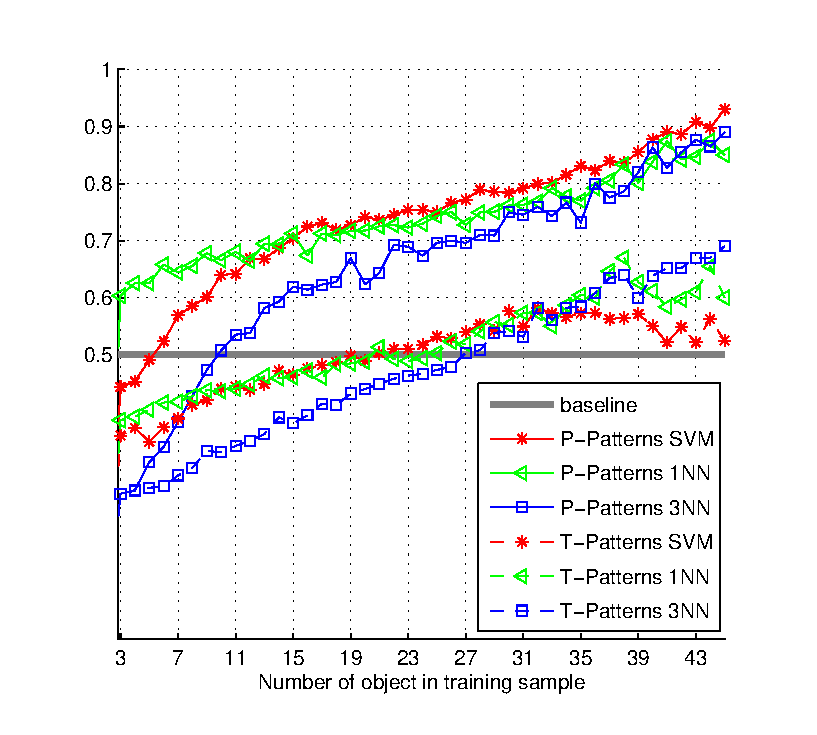
\includegraphics[width=95mm]{4classes.eps}
	\end{multicols}
	\caption{ Слева: таблица соответствий $match(i,j)$, для $MinPat=4$, $\beta=0$. Группы(слева на право): контрольная(12 элементов),
мыши без гиппокампа(12 элементов), рандомизированные данные второй группы(15 элементов), искусственные паттерны(7 элементов).
Справа: средняя доля правильных ответов классификации методами SVM, 1NN, 3NN. }
\label{fig:4classes}
\end{figure}

\subsection{Характерные паттерны}
Среди найденных паттернов можно выделить именно \emph{характерные} для определенного
класса паттерны. Неформально, паттерн является характерным для заданного класса, 
если он присутствует в поведении многих особей этого класса и редко выявляется в поведении 
животных из других классов. Для формализации данного понятия можно использовать 
Статистическое, энтропийное, или эмпирическое определение информативности~\cite{Voron_Logic}.

В~Таб.~\ref{tab:char_pat} приведены некоторые характерные паттерны для мышей из контрольной и гиппокампальной групп.


\subsection{Обсуждения и выводы}
Реализованный в данной дипломной работе метод решает поставленные перед ним задачи и производит 
качественный поиск закономерностей как в синтетических временн\'{ы}х рядах, так и в реальных
поведенческих данных. 
Предложенный метод поиска P-Паттернов имеет 2 главных недостатка:
\begin{itemize}
\item[$-$]
из-за статистической основы метода, при малых объемах данных, некоторые паттерны могут быть приняты за шум. С этим эффектом
можно бороться путем более тщательного подбора параметров алгоритма. 
\item[$-$]
Алгоритм имеет экспоненциальную сложность и, несмотря на 140-кратное ускорение, будет
крайне долго работать на очень длинных данных(на несколько порядков длиннее, чем стандартная разметка поведения мышей). 
Имеющиеся в нашем распоряжении поведенческие данные обрабатывались не дольше двух минут.Если данная проблема 
будет актуальна, ее можно решить, выставив ограничение на максимальную длину связи между событиями в паттерне.
\end{itemize}

В данной работе алгоритм поиска закономерностей рассматривался в контексте применения его для анализа поведения.
Но, очевидно, заменив понятие поведенческого акта на какое-то абстрактное событие(маркер), мы можем 
искать закономерности в различных потоках данных. Например, событиями могут быть:
повышения и понижения курсов валют в анализе поведения рынка;
аминокислоты, кодоны, или азотистые основания при анализе структуры ДНК;
всплеск активности отдельного нейрона при анализе спайковой активности нейронных культур;
новостные тренды(в виде ключевых слов) при анализе закономерностей в политике и обществе.
Например, алгоритм Т-Паттернов и ранее был использован для анализа структуры 
ДНК~\cite{TP_DNA} и стратегии футбольных команд во время матчев~\cite{TP_FOOTBALL}.



\section{Заключение}
Основные результаты работы:
\begin{itemize}
 \item Разработан метод для поиска закономерностей в последовательностях событий.
 \item Для поиска поведенческих закономерностей
 предложенный метод дает результаты, как минимум, не хуже, чем широко зарекомендовавшие себя методы.
 \item Представлены свободные, документированные реализации методов
поиска предложенного метода поиска P-Паттернов, а также метода поиска Т-Паттернов. 
\item Разработаны эффективные параллельные версии методов поиска P-Паттернов и Т-Паттернов.
\begin{itemize}
\item[$\circ$]
Пиковое ускорение для параллельной реализации поиска Т-Паттернов на 4-х ядерном \verb!CPU!~--- $3.53$ раза.
\item[$\circ$]
Пиковое ускорение для параллельной реализации процедур поиска P-Паттернов на \verb!NVIDIA GeForce8800GTX!~--- 
20 раз(этап конструирования) и 140 раз(этап подсчета правдоподобия).
\end{itemize}
\item 
Для реальных экспериментов с мышами, предложенный метод
выделяет паттерны, по которым можно определить из какой
группы была взята наблюдаемая особь. То есть, по данным о поведения особей решена задача классификации.
\end{itemize}

Система, разработанная и реализованная в данной работе, позволит биологам решать ряд практически
важных задач, возникающих при исследовании поведения: выделение поведенческих закономерностей
животных, анализ вариабельности и сложности поведения, выявление отличительных черт поведения среди разных групп 
животных, анализ спайковой активности нейронов. 
Решение этих задач позволит проводить качественный анализ влияния медицинских препаратов на поведение животных, 
связи различных анатомических структур мозга и поведения.

Дальнейшая работа в данной области будет связана, во-первых, с исследованием возможности 
расширения множества задач, которые можно решить предложенным методом. Во-вторых, планируется
разработать удобную для биологов графическую среду для исследования поведенческих закономерностей.

Автор работы выражают благодарность членам <<Лаборатории Нейробиологии Памяти>> при
Институте Нормальной Физиологии П.К.~Анохина, возглавляемой членом-корреспондентом РАН К.В.~Анохиным.
Отдельно благодарим Ирину Зарайскую, предоставившую нам экспериментальные данные по поведению.

Работа выполнена при финансовой поддержке РФФИ(проект №08-01-00405),
гранта Президента РФ(МК3827.2010.9),
и федеральной целевой программы <<Научные и научно-педагогические кадры инновационной России>>
на 2009--2013 годы(контракт №П1265).


\newpage

\addcontentsline{toc}{section}{Список литературы}
\begin{thebibliography}{00} % библиография
\bibitem{Martin_Bateson}
P.~Martin, P.~Bateson. Measuring Behaviour: An Introductory Guide.~--- Cambridge University Press, second edition, 1993.

\bibitem{Magnusson}
M.S.~Magnusson. Discovering hidden time patterns in behavior:
T-patterns and their detection.~--- Behavior Research Methods, Instruments, Computers
2000, 32 (I), 93--I IO.

\bibitem{MB_article}
V.V.~Vishnevskiy, D.P~Vetrov. The Algorithm for Detection of Fuzzy Behavioral Patterns.
~--- Proceedings of Measuring Behavior 2010,ISBN 978-90-74821-86-5.

\bibitem{Stoop}
R.~Stoop, B.~Arthur. Periodic orbit analysis demonstrates genetic constraints, variability, and switching in Drosophila courtship behavior.
~//~Chaos~--~2008~--vol.18/2.

\bibitem{POrbits}
P.~Cvitanovic. Periodic orbits as the skeleton of classical and quantum chaos.~
//~Physica D: Nonlinear Phenomena~--~1991~--~vol.51~--~Issues 1-3~--~Pp. 138--151.

\bibitem{Shurygin}
А.М.~Шурыгин. Математические методы прогнозирования.
~--- Горячая Линия~--~Телеком, 2009. ISBN   978-5-9912-0062-2.

\bibitem{NS_1}
N. Raichma, E. Ben-Jacob.
Identifying repeating motifs in the activation of synchronized bursts in cultured neuronal networks.
~//~Journal of Neuroscience Methods~--~2007~--~vol.170~--~Pp. 96–-110.

\bibitem{NS_2}
J.-M.~Fellous, P.H.E.~Tiesinga, P.J.~Thomas, T.J.~Sejnowski.
Discovering spike patterns in neuronal responses.
~//~The Journal of Neuroscience~--~March 24, 2004~--~vol.24(12)~--~Pp. 2989-–3001.


\bibitem{PPE}
Sheng Ma, J.L.~Hellerstein. Mining partially periodic event patterns with Uuknown periods.
~---~IBM T.J. Watson Research Center Hawthorne, NY 10532

\bibitem{coursework}
В.В. Вишневский, Д.П. Ветров.
Поиск скрытых поведенческих паттернов.
~---~Курсовая работа. ВМиК МГУ 2009.

\bibitem{NV_doc}
\verb!NVIDIA! Corporation.
\verb!NVIDIA CUDA!. Compute Unified Device Architecture.
~---~[\verb!PDF!]~--~2008~--~(\href{http://developer.download.nvidia.com/compute/cuda/2_0/docs/NVIDIA_CUDA_Programming_Guide_2.0.pdf}{NVIDIA\_CUDA\_Programming\_Guide\_2.0.pdf}).

\bibitem{NV_reduction}
M. Harris.
Optimizing parallel reduction in \verb!CUDA!.
~---~[\verb!PDF!]~--~(\href{http://developer.download.nvidia.com/compute/cuda/1_1/Website/projects/reduction/doc/reduction.pdf}{reduction.pdf}).


\bibitem{Boreskov_CUDA}
Б.А. Боресков, А.В. Харламов
Основы работы с технологией CUDA.
~---~ДМК Пресс, 2010~--~ISBN 978-5-94074-578-5.

\bibitem{CUDA_showcase}
\verb!CUDA! Zone.
\verb!CUDA! community showcase.
~---~[\verb!HTML/SWF!]~--~(\url{http://www.nvidia.com/object/cuda_apps_flash_new.html} ).

\bibitem{TP_DNA}
M.S.~Magnusson. Analyzing complex real-time streams of behavior:
repeated patterns in behavior and DNA.~--- L'éthologie appliquée aujourd'hui.~--~vol.3~--~Ethologie humaine. Levallois-Perret~--~France, 2003~--~ISBN 2-7237-0025-9.

\bibitem{TP_FOOTBALL}
G.K.~Jonsson, S.H.~Bjarkadottir, B.~Gislason. 
Detection of real-time patterns in sports: interactions in football.
~--- L'éthologie appliquée aujourd'hui.~--~vol.3~--~Ethologie humaine. Levallois-Perret~--~France, 2003~--~ISBN 2-7237-0025-9.

\bibitem{Neuro_exploring_the_brain}
M.F.~Bear, B.W.~Connors, M.A.~Paradiso. Neuroscience: Exploring the Brain.~--- Lippincott Williams \& Wilkins~--~3d editin, 2006.

\bibitem{Anokhin_HIP}
A.L.~Vyssotski, G.~Dell'Omo, I.I.~Poletaeva, D.L.~Vyssotski.
Long-term monitoring of hippocampus-dependent behavior in naturalistic settings: m
utant mice lacking neurotrophin receptor TrkB in the forebrain show spatial learning but impaired behavioral flexibility. 
~//~Hippocampus, 12~--~Pp. 27-–38~doi: 10.1002/hipo.10002.


\bibitem{Voron_Logic}
К.В.~Воронцов.
Лекции по логическим алгоритмам классификации.~--- 2010.

\end{thebibliography}
\newpage

\section[Приложение 1. Документация к программной реализации методов]{Приложение 1. 
Документация к программной реализации алгоритма алгоритмов поиска P-Паттернов и Т-Паттернов. Интерфейс в среде MATLAB}
Все исходные коды, бинарные пакеты, и данные могут быть запрошены по адресу \url{valera.vishnevskiy@yandex.ru}.
\subsection{Формат входных данных}
Временной ряд должен быть представлен в виде текстового файла следующего формата:
\begin{verbatim}
Time    Event
0       :
time(int)    event(string_w\o_spaces)
...
time(int)    event(string_w\o_spaces)
time(int)    &
\end{verbatim}
Обратите внимание на то, что элементы каждой строки разделены
символом табуляции \verb!\t!.

\subsection{Консольное приложение для поиска Т-Паттернов}
Консольное приложение написано на чистом \verb!C! с расширением \verb!OpenMP!, для
создания исполняемого файла использовался компилятор \verb!GCC 4.4.5(arch x86_64-linux-gnu)!. Приложение
можно запускать из консоли следующим образом:
\texttt{
\#>./t\_pattern\_core -i {\em путь\_к\_входному\_файлу} -o {\em путь\_к\_выходному\_файлу}
[-s \\{\em уровень\_значимости\_паттернов}] [-n {\em минмиальное\_число\_появления\_паттерна}]
[-q ci\_shortest|ci\_longest|ci\_most\_significant] [-e]
}

Переменная окружения \verb!OMP_NUM_THREADS! определяет количество потоков на которое
распараллеливается программаю

\subsection{Интерфейс к приложению для поиска Т-Паттернов в среде MATLAB}
\noindent
\begin{tabular}[t]{p{9em}p{29em}}
\noalign{\hrule height 2pt}
\multicolumn{2}{p{38em}}{
\vspace{1em}
\parbox{37em}{
\texttt{function [events, Nt, ts] = T\_GENERATE\_PATTERN( pat\_sym, noise\_sym, CIs, Npat, dist\_b\_patterns, Pnoise1, Pnoise2 )}
}
\vspace{1em}
}\\ 
{\bf Параметр} & {\bf Описание}\\
\noalign{\hrule height 2pt}
{\itshape Вход:} & ~ \\
\texttt{pat\_sym}& Матрица \texttt{1x$N_p$} типа \texttt{char}, определяющая паттерн. Каждый символ~--- событие. \\
\end{tabular}
\begin{tabular}[t]{p{9em}p{29em}}
\texttt{noise\_sym}& Матрица \texttt{1xN} типа \texttt{char}. Определяет события которые будут генерироваться случайно.\\
\end{tabular}
\begin{tabular}[t]{p{9em}p{29em}}
\texttt{CIs}& Матрица \texttt{($N_p$-1)x2} типа \texttt{int}. В $i$-й строке которой, записан соответствующий критический интервал.\\
\texttt{Npat}& Количество паттернов, которые требуется сгенерировать.\\
\end{tabular}
\begin{tabular}[t]{p{9em}p{29em}}
\texttt{dist\_b\_patterns}& Максимальное расстояние между двумя появлениями паттерна.\\
\end{tabular}
\begin{tabular}[t]{p{9em}p{29em}}
\texttt{P\_noise1}& Частота встречаемости шумовых символов.\\
\end{tabular}
\begin{tabular}[t]{p{9em}p{29em}}
\texttt{P\_noise2}& Вероятность того, что символ из паттерна будет зашумлен.\\
\hline
{\itshape Выход:} & ~\\
\texttt{events} &  Массив структур \texttt{1xN}, где \texttt{N}~--- количество событий. Каждая структура состоит из двух полей:
\texttt{event\_name}~--- строка названия события, и \texttt{indexes}~--- матрица \texttt{1хN} типа \texttt{int}. Определяет времеа
появления событий. \\    
\end{tabular}
\begin{tabular}[t]{p{9em}p{29em}} 
\texttt{Nt}& Продолжительность получившегося периода наблюдений.\\
\end{tabular}
\begin{tabular}[t]{p{9em}p{29em}}
\texttt{ts}& Символьная матрица \texttt{1xNt}.\\
\noalign{\hrule height 2pt}
\end{tabular}
Создает временной ряд, содержащий \verb!Npat! копий одного искусственного паттерна.

\noindent
\begin{tabular}[t]{p{9em}p{29em}}
\noalign{\hrule height 2pt}
\multicolumn{2}{p{38em}}{
\vspace{1em}
\parbox{37em}{
\texttt{function [events, Nt] = T\_LOAD\_FILE( fname )}
}
\vspace{1em}
}\\ 
{\bf Параметр} & {\bf Описание}\\
\noalign{\hrule height 2pt}
{\itshape Вход:} & ~ \\
\texttt{fname}& Путь к текстовому фалу правильного формата. \\
{\itshape Выход:} & ~\\
\texttt{events} &  Массив структур \texttt{1xN}, где \texttt{N}~--- количество событий. Каждая структура состоит из двух полей:
\texttt{event\_name}~--- строка названия события, и \texttt{indexes}~--- матрица \texttt{1хN} типа \texttt{int}. Определяет времеа
появления событий. \\    
\end{tabular}
\begin{tabular}[t]{p{9em}p{29em}} 
\texttt{Nt}& Продолжительность получившегося периода наблюдений.\\
\noalign{\hrule height 2pt}
\end{tabular}
Загружает временной ряд из текстового файла, определенного выше формата.

\noindent
\begin{tabular}[t]{p{9em}p{29em}}
\noalign{\hrule height 2pt}
\multicolumn{2}{p{38em}}{
\vspace{1em}
\parbox{37em}{
\texttt{function patterns = mexPattern( events, Nt, levels, allow\_same\_events, ci\_strategy )}
}
\vspace{1em}
}\\ 
{\bf Параметр} & {\bf Описание}\\
\noalign{\hrule height 2pt}
{\itshape Вход:} & ~ \\
\texttt{events, Nt}& Cм. определение \texttt{T\_GENERATE\_PATTERN}.\\
\end{tabular}
\begin{tabular}[t]{p{9em}p{29em}}
\texttt{levels} & Матрица \texttt{Nx3} уровней значимости. Каждая строка содержит: длину паттернов, к которым должны применяться следующие параметры; 
минимальный уровень значимости $\alpha$; минимальное количество вхождений паттерна $N_{min}$.\\
\end{tabular}
\begin{tabular}[t]{p{9em}p{29em}}
\texttt{allow\_same\_events}& 1 если, разрешается появление одинаковых событий в паттерне, 0 иначе.\\
\end{tabular}
\begin{tabular}[t]{p{9em}p{29em}}
\texttt{ci\_strategy}& Cтратегия выбора критического интервала. 
1~--- стратегия выбора длиннейшего интервала, 2~--- кратчайшего, 3~--- самого значимого.\\ 
\hline
{\itshape Выход:} & ~\\
\end{tabular}
\begin{tabular}[t]{p{9em}p{29em}}
\texttt{patterns} & Массив структур. Каждая структура описывает найденный паттерн. Поля структуры:
\texttt{Events}~--- индексы событий, которые составляют паттерн. 
\texttt{CIs}~--- интервалы, соответствующие критическим связям между событиями в паттерне.
\texttt{Sign}~--- уровень значимости найденного паттерна.
\texttt{Nab}~--- количество появлений паттерна.
\texttt{DS}~--- двойные серии({\itshape double series}) паттерна.
\texttt{String}~--- строка, описывающая паттерн в следующем формате:\\
\multicolumn{2}{c}{
$ Event_1 [dL_1, dR_1]Event_2\dots Event_m <\text{уровень значимости}> \{N_{ab}\}:(DS_1) (DS_2) \dots (DS_{N_{ab}})$ }
\\
\noalign{\hrule height 2pt}
\end{tabular}
Реализует поиск паттернов во временных рядах. 

\noindent
\begin{tabular}[t]{p{9em}p{29em}}
\noalign{\hrule height 2pt}
\multicolumn{2}{p{38em}}{
\vspace{1em}
\parbox{37em}{
\texttt{function T\_DRAW\_PATTERNS( patterns, events, Nt, np )}
}
\vspace{1em}
}\\ 
{\bf Параметр} & {\bf Описание}\\
\noalign{\hrule height 2pt}
{\itshape Вход:} & ~ \\
\texttt{patterns, events, Nt} & См. предыдущие определения.\\
\texttt{np}& Номер паттерна, который нужно представить. Или -1 для последовательного вывода всех паттернов.\\
\noalign{\hrule height 2pt}
\end{tabular}
Строит диаграмму найденных паттернов.

\noindent
\begin{tabular}[t]{p{9em}p{29em}}
\noalign{\hrule height 2pt}
\multicolumn{2}{p{38em}}{
\vspace{1em}
\parbox{37em}{
\texttt{function [p] = T\_STAT\_VALIDATE( Nt, events, levels, nvalidations )}
}
\vspace{1em}
}\\ 
{\bf Параметр} & {\bf Описание}\\
\noalign{\hrule height 2pt}
{\itshape Вход:} & ~ \\
\texttt{Nt, events, levels} & См. предыдущие определения.\\
\texttt{nvalidations} & Количество повторений процедуры рандомизации.\\
{\itshape Выход:}\\
\texttt{p} & Целочисленная матрица \texttt{1 x nvalidations}. В каждой ячейке~--- количество паттернов, найденных в рандомизированных данных.\\
\noalign{\hrule height 2pt}
\end{tabular}
Процедура статистической валидации.

\subsection{Интерфейс к приложению для поиска P-Паттернов в среде MATLAB}
Для каждого отдельного офайла определяется следующая структура параметров алгоритма. Параметры, помеченные как технические можно всегда 
оставлять заданными по-умолчанию.\\
\texttt{
conf.alpha {\em Уровень значимости паттерна $\alpha$.} [=0.001]\\
conf.kkmax {\em Выравнивание весов паттернов. Техничиский.} [=2.1]     \\
conf.Nmin  {\em Минимальное число появления паттерна $N_{min}$.} [=3]      \\
conf.lambda {\em Максимальный уровень нечеткости паттерна $\lambda$.} [=8]\\
conf.lhmult {\em Толерантность к отклонению от правдоподобия $\gamma$.} [=0.5]\\
conf.cor {\em Минимальный коэфф. корреляции $\nu$.} [=0.6]\\
conf.maxSigma {\em Максимальный тестируемый разброс.} [=round( Nt / 250 )]\\
conf.maxMu {\em Максимальное тестируемое отклонение.} [=round( Nt / 3 )]\\
conf.min\_pow\_missed {\em Степень экспоненты при пропуске. Технический.} [=-8]\\
}

\noindent
\begin{tabular}[t]{p{9em}p{29em}}
\noalign{\hrule height 2pt}
\multicolumn{2}{p{38em}}{
\vspace{1em}
\parbox{37em}{
\texttt{function [p] = T\_GENERATE\_FUZZY\_PATTERN( pat\_sym, noise\_sym, thetas, Npat, dist\_b\_patterns, Pnoise1, Pnoise2 )}
}
\vspace{1em}
}\\ 
{\bf Параметр} & {\bf Описание}\\
\noalign{\hrule height 2pt}
{\itshape Вход:} & ~ \\
\texttt{pat\_sym, noise\_sym, Npat, dist\_b\_patterns, Pnoise1, Pnoise2} & См. предыдущие определения для Т-Паттернов.\\
\texttt{thetas} & Матрица \texttt{Npat x 2} пар смещение, разброс для каждого события в паттерне.\\
{\itshape Выход:}\\
\texttt{events} &  Массив структур \texttt{1xN}, где \texttt{N}~--- количество событий. Каждая структура состоит из двух полей:
\texttt{event\_name}~--- строка названия события, и \texttt{indexes}~--- матрица \texttt{1хN} типа \texttt{int}. Определяет времеа
появления событий. \\    
\end{tabular}
\begin{tabular}[t]{p{9em}p{29em}} 
\texttt{Nt}& Продолжительность получившегося периода наблюдений.\\
\end{tabular}
\begin{tabular}[t]{p{9em}p{29em}}
\texttt{ts}& Символьная матрица \texttt{1xNt}.\\
\noalign{\hrule height 2pt}
\end{tabular}
Процедура генерация данных с нечетким паттерном.

\noindent
\begin{tabular}[t]{p{9em}p{29em}}
\noalign{\hrule height 2pt}
\multicolumn{2}{p{38em}}{
\vspace{1em}
\parbox{37em}{
\texttt{function [ps] = T\_PS\_FROM\_TS( events, Nt, sigma0, conf )}
}
\vspace{1em}
}\\ 
{\bf Параметр} & {\bf Описание}\\
\noalign{\hrule height 2pt}
{\itshape Вход:} & ~ \\
\texttt{events, Nt} & См. предыдущие определения.\\
\texttt{sigma0} & Значение разброса для псевдопаттерна. Обычно берется =1.\\
\texttt{conf} & Структура параметров, см. выше.\\
{\itshape Выход:}\\
\texttt{ps} &  Массив структур нечетких псевдопаттернов. \\    
\noalign{\hrule height 2pt}
\end{tabular}
Создание множества псевдопаттернов из временного ряда.

\noindent
\begin{tabular}[t]{p{9em}p{29em}}
\noalign{\hrule height 2pt}
\multicolumn{2}{p{38em}}{
\vspace{1em}
\parbox{37em}{
\texttt{function [ppl] = T\_FIND\_PATTERNS( events, ps, Nt, pattern\_window, use\_cuda, conf )}
}
\vspace{1em}
}\\ 
{\bf Параметр} & {\bf Описание}\\
\noalign{\hrule height 2pt}
{\itshape Вход:} & ~ \\
\texttt{events, Nt, ps, conf} & См. предыдущие определения.\\
\texttt{pattern\_window} & Технический параметр. Значение не важно.\\
\texttt{use\_cuda} & Флаг использования \texttt{GPU. true|false}.\\
{\itshape Выход:}\\
\texttt{ppl} &  Массив структур нечетких паттернов. \\    
\noalign{\hrule height 2pt}
\end{tabular}
Производит поиск закономерностей.

\newpage
\section{Приложение 2. Таблицы}
\begin{table}[H]
\centering{
\begin{tabular}{@{\vspace{-0.3cm}} |c|c||c|c| }
\hline
Число потоков & Число событий & Время работы & Ускорение  \\[1ex]
\hline
1 & 146 & 0.060 & 1.00 \\
2 & 146 & 0.030 & 2.00 \\
4 & 146 & 0.022 & 2.73 \\
8 & 146 & 0.020 & 3.00 \\
10 & 146 & 0.020 & 3.00 \\
16 & 146 & 0.020 & 3.00 \\
20 & 146 & 0.020 & 3.00 \\[1ex]
\hline
1 & 290 & 1.165 & 1.00 \\
2 & 290 & 0.650 & 1.79 \\
4 & 290 & 0.393 & 2.96 \\
8 & 290 & 0.360 & 3.24 \\
10 & 290 & 0.350 & 3.33 \\
16 & 290 & 0.330 & 3.53 \\
20 & 290 & 0.330 & 3.53 \\[1ex]
\hline
1 & 448 & 9.165 & 1.00 \\
2 & 448 & 5.950 & 1.54 \\
4 & 448 & 3.800 & 2.41 \\
8 & 448 & 2.925 & 3.13 \\
10 & 448 & 3.005 & 3.05 \\
16 & 448 & 2.685 & 3.41 \\
20 & 448 & 2.705 & 3.39 \\[1ex]
\hline
1 & 680 & 54.300 & 1.00 \\
2 & 680 & 35.580 & 1.53 \\
4 & 680 & 19.980 & 2.72 \\
8 & 680 & 17.240 & 3.15 \\
10 & 680 & 17.010 & 3.19 \\
16 & 680 & 15.800 & 3.44 \\
20 & 680 & 15.400 & 3.53 \\[1ex]
\hline
1 & 759 & 108.320 & 1.00 \\
2 & 759 & 64.845 & 1.67 \\
4 & 759 & 43.880 & 2.47 \\
8 & 759 & 34.710 & 3.12 \\
10 & 759 & 32.860 & 3.30 \\
16 & 759 & 31.240 & 3.47 \\
20 & 759 & 32.000 & 3.38 \\[1ex]
\hline
\end{tabular}}
\caption{Время работы и ускорение алгоритма поиска Т-Паттернов на 4-х ядерном процессоре.}
\label{tab:omp_tpt}
\end{table}

\begin{table}
\centering{
\begin{tabular}{@{\vspace{-0.3cm}} |c|c|c|c| }
\hline
Число точек & Время работы на \verb!CPU! & Время работы на \verb!GPU! & Ускорение  \\[1ex]
\hline
10 & 0.00 & 0.00 & 1.00 \\
100 & 0.16 & 0.01 & 14.55 \\
250 & 0.54 & 0.03 & 18.00 \\
500 & 1.54 & 0.08 & 19.25 \\
900 & 4.19 & 0.26 & 16.10 \\
1500 & 9.94 & 0.49 & 20.29 \\[2ex]
\hline
\end{tabular}}
\caption{Время работы и ускорение процедуры конструирования P-Паттернов на GPU и CPU.}
\label{tab:cu_D}
\end{table}

\begin{table}
\centering{
\begin{tabular}{@{\vspace{-0.3cm}} |c|c|c|c| }
\hline
Длина времени наблюдения & Время работы на \verb!CPU! & Время работы на \verb!GPU! & Ускорение  \\[1ex]
\hline
3213 & 0.166 & 0.002571 & 64.67 \\
6773 & 0.415 & 0.003333 & 124.37 \\
8262 & 0.437 & 0.003121 & 140.00 \\
11189 & 0.610 & 0.004340 & 140.48 \\[2ex]
\hline
\end{tabular}}
\caption{Время работы и ускорение вычисления правдоподобия P-Паттернов на GPU и CPU.}
\label{tab:cu_D}
\end{table}

\begin{table}
\centering{
\begin{tabular}{c l }
\hline
\hline
~~~~& Поведенческий акт  \\
\hline
1& Не груминг\\
2& Встряхивание телом\\
3& Вычесывание задними конечностями\\
4& Выкусывание передних конечностей\\
5& Быстрое умывание носа\\
6& Умывание нос-глаза\\
7& Вылизывание ладоней\\
8& Умывание носа\\
9& Умывание головы с ушами\\
10& Вылизывание брюха\\
11& Выкусывание боков\\
12& Вылизывание задних конечностей\\
13& Выкусывание ладоней\\
14& Выкусывание задних лап\\
15& Вылизывание гениталий\\
16& Вылизывание хвоста\\
17& Умывание глаза-нос\\
18& Вылизывание боков\\
19& Вылизывание спины\\
20& Выкусывание задних конечностей\\
21& Умывание вибрисс\\
22& Обнюхивание тела\\
23& Вылизывание передних конечностей\\
24& Умывание подбородка\\
\hline
\hline
\end{tabular}}
\caption{Кодирование поведения поведенческими актами.}
\label{tab:grooming_acts}
\end{table}

\begin{table}
\centering{
\begin{tabular}{@{\vspace{-0.3cm}} |c|c|c|c|c|c|c| }
\hline
\# объектов в обучении & PP SVM & PP 1NN & PP 3NN & TP SVM & TP 1NN & TP 3NN  \\[1ex]
\hline
3&  0.84& 0.86& 0.48&  0.59& 0.59& 0.48 \\ 
4&  0.85& 0.85& 0.62&  0.61& 0.60& 0.51 \\ 
5&  0.88& 0.89& 0.73&  0.62& 0.61& 0.55 \\ 
6&  0.88& 0.90& 0.81&  0.61& 0.62& 0.57 \\ 
7&  0.88& 0.90& 0.84&  0.65& 0.63& 0.59 \\ 
8&  0.90& 0.91& 0.85&  0.63& 0.64& 0.58 \\ 
9&  0.90& 0.93& 0.89&  0.65& 0.64& 0.61 \\ 
10&  0.90& 0.94& 0.90&  0.65& 0.64& 0.60 \\ 
11&  0.91& 0.93& 0.93&  0.66& 0.65& 0.59 \\ 
12&  0.90& 0.94& 0.93&  0.67& 0.66& 0.59 \\ 
13&  0.90& 0.93& 0.94&  0.67& 0.65& 0.58 \\ 
14&  0.90& 0.95& 0.93&  0.67& 0.67& 0.59 \\ 
15&  0.89& 0.93& 0.94&  0.67& 0.69& 0.62 \\ 
16&  0.91& 0.94& 0.94&  0.68& 0.67& 0.60 \\ 
17&  0.90& 0.94& 0.94&  0.68& 0.66& 0.60 \\ 
18&  0.89& 0.95& 0.95&  0.67& 0.65& 0.59 \\ 
19&  0.90& 0.96& 0.95&  0.70& 0.70& 0.62 \\ 
20&  0.93& 0.95& 0.96&  0.69& 0.70& 0.64 \\ 
21&  0.91& 0.96& 0.96&  0.72& 0.69& 0.62 \\ 
22&  0.92& 0.96& 0.96&  0.69& 0.66& 0.66 \\ 
23&  0.94& 0.95& 0.97&  0.72& 0.68& 0.65 \\ [2ex]
\hline
\end{tabular}}
\caption{Качество классификации при использовании разных методов классификации и разных способов выделения паттернов, 
в зависимости от количества объектов обучения. Параметры подсчета числа соответствий: $MinPat=4, \; \beta=0$.
<<PP>>~--- P-Паттерны, <<TP>>~--- Т-Паттерны.
}
\label{tab:2classes}
\end{table}

\begin{table}
\centering{
\begin{tabular}{|c|c|c|p{31em}| }
\hline
$n_c$ & $n_h$ & $I_c$ &  Паттерн в формате(смещение в секундах):   $[\,\mu_1; \sigma_1]event_1...$ \\[1ex]
\hline
12&  0& 14.81& 
$[\,0.0; 0.1]$~В лизывание~гениталий $[\,2.5; 6.2]$~Вылизывание~ладоней $[\,1.2; 7.9]$~Умывание~головы~с~ушами $[\,0.4; 5.7]$~Вылизывание~задних~конечностей 
$[\,2.6; 7.9]$~Умывание~носа \\ 
\hline
11&  0& 12.25& 
$[\,0.0; 0.1]$~Вылизывание~задних~конечностей $[\,0.4; 0.2]$~Вычесывание~задними~конечностями 
$[\,16.8; 6.4]$~Вылизывание~ладоней $[\,1.7; 4.7]$~Быстрое~умывание~носа $[\,0.2; 3.4]$~Умывание~глаза~нос  \\ 
\hline

9&  0& 8.69& 
$[\,0.0; 0.1]$~Не~груминг $[\,9.8; 1.2]$~Быстрое~умывание~носа $[\,0.6; 2.6]$~Умывание~головы~с~ушами 
$[\,0.4; 0.9]$~Вылизывание~задних~конечностей $[\,5.4; 3.7]$~Умывание~носа \\ 
\hline

0&  11& 12.25& 
$[\,0.0; 0.1]$~Быстрое~умывание~носа $[\,0.7; 1.8]$~Умывание~головы~с~ушами $[\,3.5; 9.0]$~Выкусывание~боков 
$[\,31.3; 9.0]$~Не~груминг $[\,1.4; 0.4]$~Вычесывание~задними~конечностями  \\ 
\hline

\end{tabular}}
\caption{Примеры информативных характерных паттернов. $n_c,\;n_h$~--- количество появлений данного паттерна в контрольной и гиппокампальной группе, соответственно.
$I_c$~--- статистическая информативность.
}
\label{tab:char_pat}
\end{table}


\end{document}
